%Version 3.1 December 2024
% See section 11 of the User Manual for version history
%
%%%%%%%%%%%%%%%%%%%%%%%%%%%%%%%%%%%%%%%%%%%%%%%%%%%%%%%%%%%%%%%%%%%%%%
%%                                                                 %%
%% Please do not use \input{...} to include other tex files.       %%
%% Submit your LaTeX manuscript as one .tex document.              %%
%%                                                                 %%
%% All additional figures and files should be attached             %%
%% separately and not embedded in the \TeX\ document itself.       %%
%%                                                                 %%
%%%%%%%%%%%%%%%%%%%%%%%%%%%%%%%%%%%%%%%%%%%%%%%%%%%%%%%%%%%%%%%%%%%%%

%%\documentclass[referee,sn-basic]{sn-jnl}% referee option is meant for double line spacing

%%=======================================================%%
%% to print line numbers in the margin use lineno option %%
%%=======================================================%%

%%\documentclass[lineno,pdflatex,sn-basic]{sn-jnl}% Basic Springer Nature Reference Style/Chemistry Reference Style

%%=========================================================================================%%
%% the documentclass is set to pdflatex as default. You can delete it if not appropriate.  %%
%%=========================================================================================%%

%%\documentclass[sn-basic]{sn-jnl}% Basic Springer Nature Reference Style/Chemistry Reference Style

%%Note: the following reference styles support Namedate and Numbered referencing. By default the style follows the most common style. To switch between the options you can add or remove “Numbered” in the optional parenthesis. 
%%The option is available for: sn-basic.bst, sn-chicago.bst%  
 
%%\documentclass[pdflatex,sn-nature]{sn-jnl}% Style for submissions to Nature Portfolio journals
%%\documentclass[pdflatex,sn-basic]{sn-jnl}% Basic Springer Nature Reference Style/Chemistry Reference Style
\documentclass[pdflatex,sn-mathphys-num]{sn-jnl}% Math and Physical Sciences Numbered Reference Style
%%\documentclass[pdflatex,sn-mathphys-ay]{sn-jnl}% Math and Physical Sciences Author Year Reference Style
%%\documentclass[pdflatex,sn-aps]{sn-jnl}% American Physical Society (APS) Reference Style
%%\documentclass[pdflatex,sn-vancouver-num]{sn-jnl}% Vancouver Numbered Reference Style
%%\documentclass[pdflatex,sn-vancouver-ay]{sn-jnl}% Vancouver Author Year Reference Style
%%\documentclass[pdflatex,sn-apa]{sn-jnl}% APA Reference Style
%%\documentclass[pdflatex,sn-chicago]{sn-jnl}% Chicago-based Humanities Reference Style

%%%% Standard Packages
%%<additional latex packages if required can be included here>
\usepackage[utf8]{inputenc}
\usepackage[T5]{fontenc}

\usepackage{graphicx}%
\usepackage{tikz}
\usetikzlibrary{positioning, shapes.geometric, arrows.meta}
\usepackage{multirow}%
\usepackage{amsmath,amssymb,amsfonts}%
\usepackage{amsthm}%
\usepackage{mathrsfs}%
\usepackage[title]{appendix}%
\usepackage{xcolor}%
\usepackage{textcomp}%
\usepackage{manyfoot}%
\usepackage{booktabs}%
\usepackage{algorithm}%
\usepackage{algorithmicx}%
\usepackage{algpseudocode}%
\usepackage{listings}%
%%%%



%% as per the requirement new theorem styles can be included as shown below
\theoremstyle{thmstyleone}%
\newtheorem{theorem}{Theorem}%  meant for continuous numbers
%%\newtheorem{theorem}{Theorem}[section]% meant for sectionwise numbers
%% optional argument [theorem] produces theorem numbering sequence instead of independent numbers for Proposition
\newtheorem{proposition}[theorem]{Proposition}% 
%%\newtheorem{proposition}{Proposition}% to get separate numbers for theorem and proposition etc.

\theoremstyle{thmstyletwo}%
\newtheorem{example}{Example}%
\newtheorem{remark}{Remark}%

\theoremstyle{thmstylethree}%
\newtheorem{definition}{Definition}%

\raggedbottom
%%\unnumbered% uncomment this for unnumbered level heads

\graphicspath{{../Latex_report/}}
\begin{document}

\title[Proxy-Lag Cascade Ensemble cho Dự báo Sạc Xe điện]{Proxy-Lag Cascade Ensemble: Một Kiến trúc Đa chân trời cho Dự báo Mức độ Sử dụng Trạm sạc Xe điện}

\author*[1, 2]{\fnm{Xuan-Thanh} \sur{Trinh}}\email{thanh.tx20222744@hust.edu.vn}
\author[1, 2]{\fnm{Trung-Hai} \sur{Hoang}}
\author[1, 2]{\fnm{Quang-Anh} \sur{Nguyen}}
\author[1, 2]{\fnm{Ba-Minh-Dang} \sur{Vu}}

\affil*[1]{\orgname{Trường Điện - Điện tử}}
\affil[2]{\orgname{Đại học Bách khoa Hà Nội}, \orgaddress{\city{Hà Nội}, \country{Việt Nam}}}

\abstract{Sự mở rộng nhanh chóng của cơ sở hạ tầng trạm sạc Xe điện (EV) gây ra những biến động phi tuyến tính nghiêm trọng về nhu cầu phụ tải trên lưới điện, đòi hỏi các mô hình dự báo mức độ sử dụng có độ chính xác cao. Các phương pháp dự báo truyền thống thường thất bại trong việc dự báo các đỉnh tải đột biến hoặc gặp phải hiện tượng trễ pha (phase lag) khi thực hiện dự báo đa chân trời (multi-horizon predictions). Trong bài báo này, chúng tôi đề xuất một kiến trúc Proxy-Lag Cascade Ensemble mới, lấy cảm hứng từ các nguyên lý của Điều khiển Dự báo Mô hình (Model Predictive Control - MPC). Kiến trúc này bao gồm một mô hình quỹ đạo Hai giai đoạn Dựa trên Luật (Rule-Based Two-Stage) 24 giờ và một mô hình Tinh chỉnh Vi mô (Micro-Tuner) 1 giờ. Bằng cách áp dụng phương pháp Biến đổi Lũy thừa Mục tiêu (Target Power Transformation - TPT) kết hợp với hàm Mất mát Đỉnh Tùy chỉnh (Custom Peak Loss) được thiết lập về mặt toán học, phương pháp luận của chúng tôi nắm bắt hiệu quả các đỉnh tải đột ngột trong khi ngăn chặn tuyệt đối việc rò rỉ dữ liệu. Chúng tôi chứng minh rằng các mô hình tập hợp dạng cây (tree-based ensemble models), đặc biệt là XGBoost, đạt được sai số RMSE ở mức tiên tiến nhất (state-of-the-art) là 0.0664, vượt trội hơn cả các phương pháp học sâu và các mô hình cơ sở chuỗi thời gian truyền thống. Sự liên kết lý thuyết chặt chẽ giữa quỹ đạo dự báo ở cấp độ vĩ mô và sự hiệu chỉnh linh hoạt ở cấp độ vi mô đã thiết lập một tiêu chuẩn mới cho bài toán dự báo nhu cầu Xe điện, đảm bảo tính ổn định cho các lưới điện thông minh hiện đại.}

\keywords{Xe điện, Dự báo phụ tải, XGBoost, Tăng cường đặc trưng Proxy, Trễ pha, Kiến trúc hai giai đoạn}

\maketitle

\section{Giới thiệu}\label{sec1}

Sự phát triển bùng nổ của xe điện (EV) mang đến các mô hình đỉnh tải dạng hai đỉnh (bimodal peak patterns) mang tính ngẫu nhiên và phi tuyến tính cao cho lưới điện, khiến việc dự báo chính xác mức độ sử dụng trở thành một yêu cầu cấp thiết. Tuy nhiên, một thách thức cốt lõi vẫn tồn tại trong các phương pháp dự báo hiện đại: nỗ lực đạt được độ chính xác cao thường dẫn đến việc triển khai các mạng nơ-ron sâu đòi hỏi nhiều dữ liệu \cite{eren2024comprehensive, zhu2019electric}, trong khi dữ liệu thực tế tại cấp độ trạm sạc EV lại đặc trưng bởi sự khan hiếm. Mặc dù các kiến trúc học sâu nguyên khối (monolithic) thể hiện sự xuất sắc trong môi trường dữ liệu lớn, chúng lại dễ bị quá khớp (overfitting) nghiêm trọng và tốn kém tài nguyên tính toán khi đối mặt với các tập dữ liệu có kích thước nhỏ. Ngược lại, các mô hình tập hợp dựa trên cây (ensemble tree-based models) như XGBoost và Random Forest đã chứng minh được khả năng tổng quát hóa vượt trội và tính mạnh mẽ trong môi trường dữ liệu nhỏ \cite{lu2021comparative, wang2020ensemble, shahriar2020machine}. Điều này tạo ra một động lực bắt buộc phải chuyển hướng từ các mạng nơ-ron phức tạp sang các thuật toán dạng bảng (tabular algorithms) hiệu quả hơn, đóng vai trò như nền tảng cho việc dự báo phụ tải EV.

Mặc dù các mô hình dựa trên cây có nhiều ưu điểm về mặt thuật toán, các kỹ thuật hồi quy tiêu chuẩn về bản chất thường tối ưu hóa cho các chỉ số hướng giá trị trung bình (mean-seeking metrics) như Sai số Toàn phương Trung bình (MSE), dẫn đến sự đánh giá thấp có tính hệ thống đối với các đỉnh tải cực đại. Để giải quyết vấn đề này, nhiều nhà nghiên cứu đã sử dụng các kỹ thuật thao tác không gian đầu vào (input-space manipulation) như SMOGN để lấy mẫu vượt mức (oversample) cho các dữ liệu đỉnh tải thiểu số. Tuy nhiên, những phương pháp tăng cường dữ liệu nhân tạo như vậy làm biến dạng không thể khắc phục phân phối cơ bản của các đặc trưng phân loại (categorical features), làm tổn hại đến khả năng diễn giải vật lý của dữ liệu. Thay vào đó, các tiến bộ gần đây ủng hộ mạnh mẽ các can thiệp trong không gian đầu ra (output-space interventions), chứng minh rằng các hàm mất mát bất đối xứng và tùy chỉnh \cite{wu2021support, ko2025deterministic, kim2026methodology} khi kết hợp với kiến thức chuyên ngành có thể phạt nặng lỗi dự báo thấp (under-forecasting) mà không làm suy giảm tính toàn vẹn của dữ liệu. Điều này củng cố việc chuyển hướng sang sử dụng Biến đổi Lũy thừa Mục tiêu (TPT) và các hàm mất mát tùy chỉnh. Tuy nhiên, việc nắm bắt các đỉnh tải cực đại về mặt toán học lại làm giảm đi độ chính xác tại các thung lũng phụ tải (off-peak valleys), cho thấy rằng một mô hình nguyên khối duy nhất không thể làm chủ đồng thời cả hai thái cực này.

Sự đánh đổi nội tại giữa độ nhạy tại đỉnh và độ ổn định tại thung lũng đòi hỏi một phương pháp tiếp cận "chia để trị" (divide-and-conquer) về mặt cấu trúc. Các phương pháp luận truyền thống thường đưa ra một bộ phân loại (classifier) độc lập để dự đoán sự xuất hiện của các đỉnh, từ đó kích hoạt một mô hình chuyên biệt cho đỉnh tải. Tuy nhiên, cách tiếp cận này tạo ra gánh nặng tính toán đáng kể, đòi hỏi phải duy trì nhiều mô hình riêng biệt và làm trầm trọng thêm sự lan truyền sai số (error propagation). Một giải pháp tinh tế hơn nhiều nằm ở kiến trúc phân cấp hai giai đoạn \cite{laouafi2016daily, hsu2018two}, nơi các bộ kích hoạt dựa trên luật vật lý (physical rule-based triggers) phân chia không gian dự báo mà không chịu gánh nặng của một bộ phân loại độc lập. Bằng cách cô lập các hành vi khắc nghiệt khỏi đường cơ sở chính \cite{chen2019short, rubasinghe2023highly, papadakis1998novel}, cơ chế phân đoạn dựa trên luật có thể chuyển đổi mượt mà giữa một mô hình thung lũng ổn định và một mô hình nắm bắt đỉnh cực đại dựa trên các ngưỡng sử dụng cụ thể, qua đó bảo toàn sự tinh giản của mô hình và tối ưu hóa hiệu suất tính toán.

Ngay cả khi việc tách biệt đỉnh và thung lũng trong 24 giờ diễn ra hoàn hảo, dự báo đa chân trời về bản chất vẫn phải chịu một điểm mù ở cấp độ vĩ mô, khiến các biến động ở cấp độ vi mô kích hoạt hiện tượng trễ pha nghiêm trọng---một hiện tượng mà trong đó các dự đoán liên tục theo sau các sự kiện thực tế một bước thời gian (time step). Những nỗ lực giải quyết vấn đề này chỉ bằng cách thu hẹp chân trời dự báo xuống các khoảng thời gian 1 giờ bằng cách sử dụng các đặc trưng động học (kinematic features) hoặc nắn chỉnh thời gian động (dynamic time warping) đều liên tục thất bại, vì các mô hình dạng cây tại từng điểm (point-wise tree models) không thể hiểu được các động lực ở cấp độ chuỗi (sequence-level dynamics). Thay vào đó, bước đột phá nằm ở học phần dư (residual learning) và các kiến trúc hiệu chỉnh sai số \cite{kong2020short, shen2020novel}. Bằng cách sử dụng một mô hình quỹ đạo cơ sở để thiết lập một proxy có tính chu kỳ và giới hạn mô hình vi mô 1 giờ trong việc dự đoán mục tiêu tuyệt đối thông qua việc tận dụng proxy \cite{zhang2021novel}, quán tính của hiện tượng trễ pha trong chuỗi thời gian bị triệt tiêu một cách hiệu quả. Cơ chế xếp tầng (cascade) này mô phỏng triết lý của Điều khiển Dự báo Mô hình (MPC), sử dụng một proxy vĩ mô 24 giờ để dẫn dắt bộ hiệu chỉnh vi mô 1 giờ.

Để giải quyết những thách thức mang tính phức hợp này, bài báo đề xuất Proxy-Lag Cascade Ensemble---một kiến trúc được thiết kế tỉ mỉ, kết hợp Biến đổi Lũy thừa Mục tiêu, phân nhánh dựa trên luật, và hiệu chỉnh sai số phần dư. Các đóng góp của chúng tôi bao gồm ba điểm chính: (1) Đề xuất mô hình cơ sở Hai giai đoạn Dựa trên Luật cho chân trời dự báo $t+24$ tinh tế về mặt toán học, được dẫn dắt bởi một hàm Mất mát Đỉnh Tùy chỉnh, hoàn toàn loại bỏ các phương pháp tăng cường đầu vào gây biến dạng dữ liệu cũng như các bộ phân loại làm cồng kềnh hệ thống; (2) Giới thiệu một Bộ Tinh chỉnh Vi mô (Micro-Tuner) $t+1$ tích hợp một cách rõ ràng proxy vĩ mô vào việc dự đoán mục tiêu tuyệt đối nhằm phá vỡ hoàn toàn hiện tượng trễ pha phổ biến; và (3) Xây dựng một khuôn khổ khái niệm lấy cảm hứng từ MPC, chứng minh cách thức các hiệu chỉnh vi mô ngắn hạn $1$ giờ bổ sung và củng cố hiệu quả cho quỹ đạo dự báo vĩ mô $24$ giờ, thu hẹp khoảng cách giữa khả năng dự báo vĩ mô và sự linh hoạt vi mô, qua đó tạo ra một mô hình dự báo sử dụng EV mạnh mẽ.

Phần còn lại của bài báo được cấu trúc như sau: Mục \ref{sec2} trình bày chi tiết các bước tiền xử lý dữ liệu và khuôn khổ toán học của phương pháp luận được đề xuất, bao gồm hàm Mất mát Đỉnh Tùy chỉnh, kiến trúc Hai giai đoạn Dựa trên Luật, và Proxy-Lag Cascade Ensemble. Mục \ref{sec3} giới thiệu thiết lập thực nghiệm, trực quan hóa các hành vi lý thuyết, và cung cấp một cuộc thảo luận so sánh toàn diện về các kết quả. Cuối cùng, Mục \ref{sec4} kết luận bài báo.

\section{Vật liệu và Phương pháp nghiên cứu}\label{sec2}

\subsection{Case Study: EV Station 00015}
Nghiên cứu này khai thác bộ dữ liệu quy mô lớn "EV charging station availability tracking" công bố trên nền tảng Kaggle\footnote{Kaggle: Tập dữ liệu EV charging station availability tracking}. Bộ dữ liệu ghi nhận trạng thái khả dụng của hệ thống cung cấp điện cho xe điện (EVSE) trên toàn bộ một mạng lưới trạm sạc rộng lớn theo chuỗi thời gian có độ phân giải cao. Ở cấp độ vĩ mô, dữ liệu phản ánh sự tương tác động giữa hạ tầng sạc và hành vi người dùng, bao gồm các mô hình không gian-thời gian, sự tắc nghẽn vào giờ cao điểm, và nhu cầu di chuyển trong đô thị. Trong mạng lưới rộng lớn này, các trạm sạc thể hiện tần suất sử dụng và độ biến động hoàn toàn khác nhau tùy thuộc vào vị trí (khu dân cư, trung tâm thương mại, v.v.).

Để đánh giá nghiêm ngặt năng lực dự báo và độ vững của khung mô hình được đề xuất, nghiên cứu đã chuyển từ phân tích mạng lưới vĩ mô sang tập trung vào cấp độ vi mô. Cụ thể, Trạm sạc EV 00015 đã được cô lập và chọn làm Case Study cốt lõi. Lý do lựa chọn EV 00015 nằm ở hồ sơ tải (load profile) cực kỳ phức tạp của nó: tính phi tập trung cao, độ biến động mạnh, và đặc biệt là phân bố dạng bimodal (hai đỉnh). Khác với các trạm thông thường có chu kỳ ngày/đêm dễ dự đoán, EV 00015 chứa các gai (spikes) sử dụng bất quy tắc và độ nhiễu lớn. Do đó, việc dự báo thành công tỷ lệ khả dụng tại nút thắt này đóng vai trò như một bài kiểm tra sức chịu đựng (stress test) khắc nghiệt, minh chứng rằng kiến trúc lai đề xuất hoàn toàn có khả năng thích ứng với những thành phần khó lường nhất trong lưới điện thông minh.

\begin{figure}[h]
\centering
\resizebox{\textwidth}{!}{%
\begin{tikzpicture}[
    box/.style={draw, rectangle, minimum width=2.5cm, minimum height=1cm, align=center, fill=blue!5, rounded corners},
    arrow/.style={->, thick, >=Stealth}
]
% Nodes
\node (input) at (0, 0) {\textbf{Đặc trưng Đầu vào}};
\node[box] (base) at (3.5, 0) {Mô hình Cơ sở 24h \\ (Quỹ đạo)};
\node[box, fill=yellow!10] (trigger) at (7.5, 0) {Bộ kích hoạt dựa trên Luật \\ ($\hat{y}_{base} \ge 0.55$)};
\node[box, fill=red!10] (tpt) at (7.5, 2.5) {Mô hình TPT + \\ Hàm mất mát Tùy chỉnh};
\node[box] (proxy) at (11.5, 0) {Đặc trưng Đại diện \\ ($\hat{y}_{24h\_proxy}$)};
\node[box, fill=green!10] (corrector) at (11.5, -2.5) {Bộ tinh chỉnh Vi mô 1h \\ (Tuyệt đối)};
\node[align=center] (output) at (11.5, -4.5) {\textbf{Đầu ra Cuối cùng} \\ ($\hat{y}_{final}$)};

% Arrows
\draw[arrow] (input) -- (base);
\draw[arrow] (base) -- (trigger);
\draw[arrow] (trigger) -- node[left] {Có} (tpt);
\draw[arrow] (tpt) -| (proxy);
\draw[arrow] (trigger) -- node[above] {Không} (proxy);
\draw[arrow] (proxy) -- (corrector);
\draw[arrow] (corrector) -- (output);
\draw[arrow] (input) |- (corrector);
\end{tikzpicture}%
}
\caption{Kiến trúc Kết hợp Chuỗi Proxy-Lag (Proxy-Lag Cascade Ensemble Architecture). Hệ thống phân nhánh dự báo vĩ mô 24 giờ sử dụng một bộ kích hoạt dựa trên luật, sau đó thiết lập một biến đại diện (proxy) có tính chu kỳ nhằm định hướng bộ tinh chỉnh vi mô 1 giờ.}
\label{fig:architecture}
\end{figure}

\subsection{Tiền xử lý Dữ liệu và Trích xuất Đặc trưng}\label{subsec2_1}

Tập dữ liệu chính được sử dụng trong nghiên cứu này là ACN-Data (Adaptive Charging Network Data), một tập dữ liệu mã nguồn mở chứa thông tin về các phiên sạc xe điện trong thế giới thực. Cụ thể, dữ liệu của chúng tôi bao trùm nhiều tháng hoạt động liên tục tại một số trạm sạc có lưu lượng cao. Điều cốt lõi là biến mục tiêu---tỷ lệ sử dụng trạm ($y$)---được định nghĩa là tỷ lệ giữa số lượng phiên sạc đang hoạt động trên tổng công suất của trạm. Định nghĩa này giới hạn biến mục tiêu trong khoảng $[0, 1]$, trong đó 0 biểu thị trạm đang rảnh rỗi và 1 biểu thị trạm đạt công suất tối đa. Việc giới hạn này cung cấp bối cảnh cho các số đo sai số tiếp theo (ví dụ: RMSE), gắn liền hiệu suất với các ràng buộc vật lý. 

Tập dữ liệu hoạt động thô, được ghi lại ở độ phân giải tần số cao 30 phút, bộc lộ các nhiễu cục bộ thường che khuất các xu hướng vĩ mô rộng lớn hơn của nhu cầu sạc xe điện. Để thiết lập một cơ sở mô hình hóa ổn định, chúng tôi áp dụng chiến lược tổng hợp thời gian có cấu trúc, hạ lấy mẫu (down-sampling) độ phân giải thời gian xuống các khoảng thời gian 1 giờ. Quá trình lấy mẫu lại này áp dụng các phép tổng hợp cụ thể được tinh chỉnh cho ý nghĩa vật lý của từng lớp đặc trưng. Các biến liên tục, chẳng hạn như tỷ lệ sử dụng và nhiệt độ môi trường, được tổng hợp thông qua trung bình cộng để bảo toàn độ lớn đại diện của chúng. Ngược lại, các chỉ báo sự kiện dạng boolean---chẳng hạn như cờ đánh dấu cuối tuần hoặc cờ giờ cao điểm---được tổng hợp sử dụng toán tử max logic, đảm bảo rằng sự xuất hiện của các sự kiện quan trọng trong vòng một giờ được bảo toàn. Hơn nữa, các đặc trưng phân loại, bao gồm điều kiện thời tiết cục bộ, được lấy mẫu bằng cách trích xuất trạng thái quan sát đầu tiên trong cửa sổ thời gian, duy trì tính liên tục của phân loại.

Sau quá trình đồng bộ hóa thời gian này, quy trình trích xuất đặc trưng (feature engineering) nghiêm ngặt được thực hiện để xây dựng một không gian trạng thái dự đoán toàn diện. Dự báo chuỗi thời gian hiệu quả dựa trên việc nắm bắt động học thời gian (temporal kinematics) và quán tính lịch sử của biến mục tiêu. Để định lượng bộ nhớ ngắn hạn tức thời và quỹ đạo của hệ thống, chúng tôi trích xuất các đặc trưng độ trễ rõ ràng (explicit lag features) tại thời điểm $t-1$ và $t-2$. Hơn nữa, để nắm bắt các hành vi chu kỳ ngày đêm bị chi phối bởi thói quen đi lại của con người, độ trễ lịch sử 24 giờ ($t-24$) được tích hợp như một mỏ neo chu kỳ vĩ mô. Vượt ra ngoài các tọa độ lịch sử theo điểm này, mô hình dự đoán cũng phải hiểu được động lượng cơ bản của các xu hướng sử dụng. Để đạt được điều này, các đặc trưng trung bình trượt (rolling mean) được tính toán trên các cửa sổ $3$ giờ và $6$ giờ được thêm vào tập dữ liệu. Các thống kê trượt này hoạt động như các bộ lọc thông thấp (low-pass filters), triệt tiêu sự biến động ngẫu nhiên và cung cấp cho các thuật toán động lượng định hướng của phụ tải sạc. Việc trích xuất toàn diện các độ trễ động học và các vector động lượng này trang bị cho các thuật toán phía sau một bối cảnh thời gian mang tính mô tả.

Để đảm bảo đánh giá mô hình một cách mạnh mẽ, tập dữ liệu chuỗi thời gian được phân chia theo trình tự thời gian thành các tập Huấn luyện (Training), Xác thực (Validation) và Kiểm tra (Testing) với tỷ lệ 70-15-15. Tập Xác thực phục vụ cho việc tinh chỉnh siêu tham số (hyperparameter) bằng Optuna và để thiết lập Tỷ lệ Kết hợp toán học (Ensemble Ratio) (33\% vĩ mô, 67\% vi mô) được sử dụng trong chuỗi. Hơn nữa, chuẩn hóa đặc trưng thông qua MinMax scaling cũng được áp dụng. Đây là một yêu cầu kỹ thuật nhằm ngăn chặn các biến có độ lớn cao thống trị các bước phân chia cây (tree-splits) và tạo ra sự ổn định số học cần thiết cho Hàm mất mát Tùy chỉnh (Custom Loss Function).



\subsection{Cơ sở Toán học của việc Bắt Đỉnh (Peak Catching): Hàm mất mát Tùy chỉnh và Chuyển đổi Lũy thừa Mục tiêu (TPT)}\label{subsec2_3}

Để tránh các tác động có hại của việc thao tác trên không gian đầu vào, chẳng hạn như thuật toán SMOGN, vốn làm biến dạng tính liên tục vật lý của các biến phân loại, phương pháp của chúng tôi chuyển hướng can thiệp một cách triệt để vào các không gian đầu ra và không gian hàm mục tiêu. Chúng tôi đề xuất phép Chuyển đổi Lũy thừa Mục tiêu (Target Power Transformation - TPT) để làm cho mô hình nhạy cảm về mặt toán học đối với các giá trị đỉnh cực đoan mà không thay đổi phân phối đầu vào. TPT được định nghĩa bằng cách lập phương tỷ lệ sử dụng mục tiêu:
\begin{equation}
y' = y^3
\end{equation}
trong đó $y$ là tỷ lệ sử dụng ban đầu và $y'$ là mục tiêu đã được chuyển đổi. Trong quá trình suy luận, các dự báo được đưa trở lại thang đo vật lý ban đầu bằng phép biến đổi ngược:
\begin{equation}
y = \text{sgn}(y') \sqrt[3]{\vert y' \vert}
\end{equation}
Việc căn chỉnh phi tuyến tính (non-linear scaling) này mở rộng đáng kể khoảng cách toán học giữa các giá trị đỉnh và thung lũng, buộc các cây gradient boosting phải ưu tiên dự báo các mức tăng đột biến. 

Để thúc đẩy hơn nữa việc tối ưu hóa thuật toán hướng tới việc bắt các đỉnh, chúng tôi xây dựng một Hàm mất mát Đỉnh Tùy chỉnh (Custom Peak Loss) dựa trên Sai số Toàn phương Trung bình có Trọng số (Weighted Mean Squared Error - WMSE). MSE tiêu chuẩn phạt các sai số một cách đồng đều trên toàn bộ miền giá trị, dẫn đến thất bại có hệ thống đối với các sự kiện cực đoan thưa thớt. Hàm mất mát Đỉnh Tùy chỉnh của chúng tôi áp đặt về mặt toán học một hình phạt khổng lồ một cách nghiêm ngặt lên các trường hợp đỉnh. Cụ thể, nó được công thức hóa bằng toán học như một dạng WMSE dựa trên ngưỡng:
\begin{equation}
\mathcal{L}_{WMSE} = \frac{1}{N} \sum_{i=1}^{N} w_i \left( y'_i - \hat{y}'_i \right)^2
\end{equation}
trong đó trọng số phạt động $w_i$ được điều chỉnh bởi ngưỡng tới hạn $0.343$:
\begin{equation}
w_i = \begin{cases} 50.0, & \text{nếu } y'_i \ge 0.343 \\ 1.0, & \text{ngược lại} \end{cases}
\end{equation}
Bởi vì $0.7^3 = 0.343$, ngưỡng này nhắm chính xác vào chế độ hoạt động tới hạn nơi mà tỷ lệ sử dụng ban đầu $y$ đạt tới $0.7$ (hoặc 70\%). Đáng chú ý là, các tham số cụ thể này---định nghĩa ngưỡng $0.7$ cho một đỉnh cực đoan và trọng số phạt khổng lồ $50.0$---không được giả định theo kinh nghiệm. Chúng được xác định một cách nghiêm ngặt thông qua framework tối ưu hóa siêu tham số Optuna bằng cách thực hiện tìm kiếm toàn diện trên tập Xác thực, đảm bảo rằng chúng đại diện cho các mức tối ưu toán học cho phân phối dữ liệu nhỏ cụ thể này. Bằng cách neo đậu hình phạt $50.0\times$ được tối ưu hóa này một cách nghiêm ngặt vào ngưỡng $y \ge 0.343$, thuật toán bị ép buộc một cách rõ ràng phải ánh xạ quyết liệt động học cơ sở của các sự kiện sạc cực đoan, do đó khắc phục các hạn chế hướng tới trung bình của hồi quy truyền thống mà không làm ảnh hưởng đến tính toàn vẹn của dữ liệu đầu vào.

\subsection{Vượt qua Thung lũng: Kiến trúc Hai Giai đoạn dựa trên Luật}\label{subsec2_4}

Mặc dù việc tích hợp TPT và Hàm mất mát Đỉnh Tùy chỉnh giải quyết một cách xuất sắc tình trạng dự báo thấp kinh niên đối với các đỉnh cực đoan, nhưng nó mang lại một hệ quả toán học: mô hình bắt đỉnh quyết liệt vốn dĩ làm mất ổn định các dự báo trong các thung lũng ổn định, ngoài giờ cao điểm. Để tổng hợp một dự báo tối ưu toàn cục, yêu cầu bắt buộc về mặt toán học là phải tách biệt chế độ thung lũng ổn định khỏi chế độ đỉnh biến động. 

Một cách tiếp cận phổ biến trong các tài liệu hiện đại là triển khai một Bộ phân loại Học máy độc lập để dự đoán sự xuất hiện của các đỉnh và sau đó chuyển đổi mô hình. Tuy nhiên, chúng tôi cực lực bác bỏ phương pháp này dựa trên nguyên lý Dao cạo Occam (Occam's Razor). Việc đưa vào một bộ phân loại độc lập, tự chủ sẽ gây ra sự phình to nghiêm trọng của hệ thống, đòi hỏi phải duy trì các quy trình trích xuất đặc trưng riêng biệt và tất yếu dẫn đến các sai số phân loại dây chuyền khi một dương tính giả kích hoạt một dự báo đỉnh quyết liệt trong một thung lũng bằng phẳng. 

Thay vào đó, chúng tôi đề xuất một Kiến trúc Hai Giai đoạn dựa trên Luật tinh gọn và khép kín. Chúng tôi sử dụng mô hình hồi quy cơ sở ổn định, không chuyển đổi làm bộ kích hoạt vật lý, loại bỏ hoàn toàn sự cần thiết của một bộ phân loại bên ngoài. Kiến trúc này hoạt động thông qua một hàm xác định từng khoảng (deterministic piecewise function), định nghĩa một Chuyển đổi Cứng Kích hoạt từ Cơ sở (Base-Triggered Hard Switch):
\begin{equation}
\hat{y}_{final} = 
\begin{cases} 
\hat{y}_{tpt} & \text{nếu } \hat{y}_{base} \ge 0.55 \\ 
\hat{y}_{base} & \text{ngược lại} 
\end{cases}
\end{equation}
Ở đây, $\hat{y}_{base}$ đại diện cho dự báo từ mô hình cơ sở tiêu chuẩn được tối ưu hóa cho sự ổn định tổng thể, và $\hat{y}_{tpt}$ là dự báo từ mô hình bắt đỉnh quyết liệt. Ngưỡng kích hoạt vật lý được đặt nghiêm ngặt ở mức $0.55$. Cụ thể, ngưỡng $0.55$ (tỷ lệ sử dụng 55\%) này không được chỉ định một cách tùy ý; nó được suy xuất một cách nghiêm ngặt thông qua một phương pháp Tìm kiếm Lưới (Grid Search) toàn diện trên tập Xác thực, xác định chính xác "điểm uốn" (inflection point) toán học nơi mà trạm sạc xe điện chuyển đổi về mặt bản chất từ trạng thái hoạt động ổn định sang trạng thái quá tải cực đoan và biến động. Nếu mô hình cơ sở xác định rằng quỹ đạo đang đi vào trạng thái sử dụng cao này ($\ge 0.55$), kiến trúc sẽ ngay lập tức thực hiện chuyển đổi cứng để xuất ra dự báo $\hat{y}_{tpt}$ quyết liệt. Ngược lại, trong các giai đoạn thung lũng ổn định, mô hình cơ sở vẫn nắm quyền kiểm soát, xuất ra $\hat{y}_{base}$. Kiến trúc này duy trì sự đơn giản của nguyên lý Dao cạo Occam, ngăn ngừa các lỗi thuật toán lũy kế và đảm bảo sự chuyển đổi toán học mượt mà giữa sự ổn định của thung lũng và độ nhạy của đỉnh.

Mặc dù kiến trúc Hai Giai đoạn giải quyết một cách xuất sắc xung đột giữa các đỉnh và thung lũng, nó về cơ bản vẫn bị neo vào một chân trời dự báo 24 giờ. Chân trời dài này tạo ra một "điểm mù" dưới dạng độ trễ pha (phase lag) hoặc không có khả năng dự đoán các biến động vi mô. Trong khi mô hình có thể dự đoán quỹ đạo vĩ mô chung của một đỉnh sắp tới, nó lại gặp khó khăn trong việc điều chỉnh các sai lệch vi mô tức thời, chẳng hạn như khi một đỉnh dịch chuyển ngoài dự kiến từ 1-2 giờ. Hệ quả là, hạn chế vốn có này của chân trời 24 giờ hoàn toàn bắt buộc phải giới thiệu một Bộ tinh chỉnh Vi mô (Micro-Tuner) ở cấp độ vi mô, đóng vai trò là pha cuối cùng trong hệ thống Proxy-Lag Cascade của chúng tôi.

\subsection{Kết hợp Proxy-Lag Cascade: Dung hợp các Chân trời Vĩ mô và Vi mô}\label{subsec2_5}

Để xóa bỏ hoàn toàn độ trễ pha vốn có trong chân trời dự báo 24 giờ, chúng tôi giới thiệu Mô hình Kết hợp Proxy-Lag Cascade, một kiến trúc được lấy cảm hứng sâu sắc từ triết lý Điều khiển Dự báo Mô hình (Model Predictive Control - MPC). Trong MPC truyền thống, một quỹ đạo vĩ mô dài hạn được thiết lập để đảm bảo sự ổn định toàn cục, trong khi các hành động điều khiển ngắn hạn cung cấp sự nhanh nhẹn tức thời nhằm loại bỏ các nhiễu loạn cục bộ. Chúng tôi chuyển hóa trực tiếp hệ hình này vào lĩnh vực dự báo phụ tải xe điện. Mô hình Hai Giai đoạn 24 giờ hoạt động như "Quỹ đạo Vĩ mô" ("Macro-Trajectory" hay Proxy). Nó sở hữu bộ nhớ chu kỳ dài hạn vượt trội và thiết lập hiệu quả hành vi cơ sở rộng lớn của trạm sạc. Tuy nhiên, vì chân trời dự báo của nó được mở rộng, nó tự nhiên phải chịu một "điểm mù" về thời gian---một sự bất lực nội tại trong việc thích ứng nhanh chóng với các thay đổi vi mô theo từng giờ đối với nhu cầu sử dụng, điều được biểu hiện về mặt toán học như độ trễ pha.

Để giải quyết hạn chế này mà không loại bỏ sự ổn định của quỹ đạo vĩ mô, chúng tôi thiết kế một Bộ tinh chỉnh Vi mô 1 giờ hoạt động như một "Micro-Tuner". Điều cốt lõi là, mô hình 1 giờ này hoàn toàn được giải phóng khỏi gánh nặng dự đoán tính mùa vụ theo ngày đêm cơ bản. Thay vào đó, bằng cách bóc tách về mặt toán học quỹ đạo cơ sở, bộ hiệu chỉnh vi mô 1 giờ cô lập và tích hợp một cách chặt chẽ dự báo 24 giờ như một \textit{Đặc trưng Đại diện} (Proxy Feature) quan trọng $P_t$, được định nghĩa là:
\begin{equation}
P_t = \hat{y}_{24h\_proxy, t}
\end{equation}
Không gian dự đoán cuối cùng do đó được chuyển đổi, nơi bộ tinh chỉnh vi mô xấp xỉ $\hat{y}_{1h\_micro} = f(X_t \cup \{P_t\})$. Bằng cách đưa rõ ràng biến đại diện vào không gian đặc trưng, Bộ tinh chỉnh Vi mô đạt được phản xạ nhanh như chớp, cho phép nó hiệu chỉnh quyết liệt các sự dịch chuyển thời gian 1 giờ và các cú sốc nhu cầu cục bộ mà mô hình 24 giờ vốn dĩ bỏ lỡ.

Hơn nữa, một ràng buộc kiến trúc quan trọng được áp đặt trong quá trình xây dựng $X_t$ cho Bộ tinh chỉnh Vi mô nhằm giảm thiểu nghiêm ngặt tình trạng Rò rỉ Dữ liệu (Data Leakage). Trong các hoạt động thực tế, dữ liệu ngoại sinh thời gian thực hoàn hảo (ví dụ: điều kiện thời tiết tức thời hoặc chỉ số giao thông) hiếm khi có sẵn ngay lập tức. Để mô phỏng tính thực tế hoạt động nghiêm ngặt này, tất cả các biến ngoại sinh được đưa vào Bộ tinh chỉnh Vi mô 1 giờ đều phải chịu một phép Dịch chuyển Ngây thơ (Naive Shift) nghiêm ngặt 24 giờ ($t-24$). Ràng buộc có chủ ý này buộc mô hình 1 giờ phải hoạt động "mù quáng" đối với các điều kiện môi trường tức thời của giờ mục tiêu. Do đó, điều này chứng minh rằng việc loại bỏ độ trễ pha được thúc đẩy thuần túy bởi tính mạnh mẽ toán học của Đặc trưng Đại diện và động học sử dụng tức thời, thay vì các tương quan giả với dữ liệu ngoại sinh thời gian thực hoàn hảo.

Sự tổng hợp kiến trúc cuối cùng kết hợp hai chân trời bổ sung này thông qua một chuỗi được tính trọng số bằng toán học. Dự báo tổng thể là một tổ hợp tuyến tính của sự ổn định cấu trúc do Quỹ đạo Vĩ mô cung cấp và sự bù trừ sai số linh hoạt do Bộ tinh chỉnh Vi mô cung cấp. Trọng số của tổ hợp tuyến tính này không được chọn theo kinh nghiệm. Chúng tôi đã thực hiện một phép tối ưu hóa Optuna toàn diện trên tập Xác thực, quét tỷ lệ kết hợp từ $0.1$ đến $0.9$. Sự hội tụ của thuật toán đã chứng minh một cách thuyết phục rằng trạng thái cân bằng toán học tối ưu---Tỷ lệ Kết hợp Vàng mang lại RMSE Xác thực thấp nhất---được công thức hóa là:
\begin{equation}
\hat{y}_{final} = 0.33 \times \hat{y}_{24h} + 0.67 \times \hat{y}_{1h\_micro}
\end{equation}
trong đó $\hat{y}_{24h}$ đại diện cho dự báo thu được từ proxy cơ sở Hai Giai đoạn 24 giờ, và $\hat{y}_{1h\_micro}$ đại diện cho đầu ra tuyệt đối từ Bộ tinh chỉnh Vi mô 1 giờ. Bằng cách gán về mặt toán học $33\%$ trọng số dự đoán cho bộ nhớ dài hạn và $67\%$ cho độ linh hoạt của phản xạ ngắn hạn, Mô hình Kết hợp Proxy-Lag Cascade đạt được sự cân bằng sâu sắc. Công thức này đảm bảo rằng hệ thống vẫn được neo vững chắc vào xu hướng chu kỳ vĩ mô, đồng thời sở hữu độ đàn hồi vi mô cần thiết để loại bỏ tức thì sự biến động ngẫu nhiên ngay lập tức, do đó thiết lập một cơ chế dự báo đặc biệt mạnh mẽ cho các lưới điện thông minh hiện đại.

\begin{figure}[ht]%
\centering
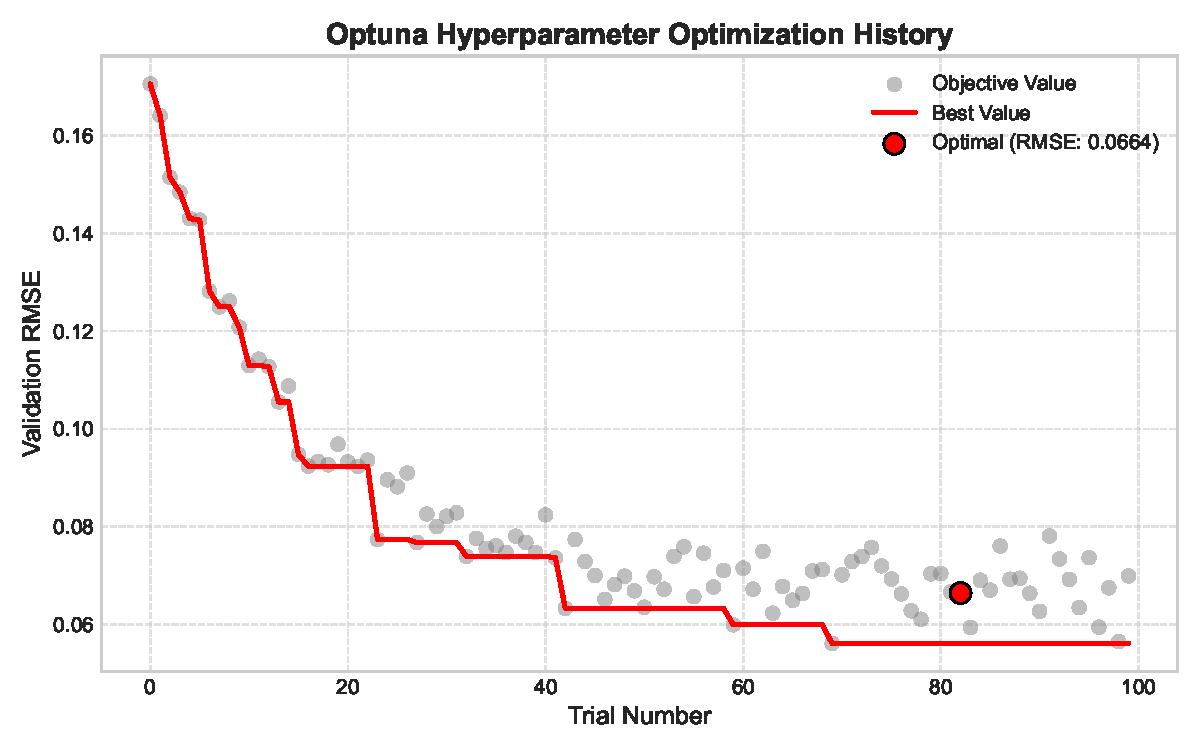
\includegraphics[width=0.8\textwidth]{images/optuna_history.pdf}
\caption{Lịch sử Tối ưu hóa Siêu tham số Optuna. Biểu đồ phân tán (scatter plot) trực quan hóa sự hội tụ của hàm mục tiêu (RMSE Xác thực) qua 100 lần thử, thiết lập một cách nghiêm ngặt các cấu hình tham số tối ưu (ví dụ: Tỷ lệ Kết hợp Vàng) và chứng minh rằng chúng là các giá trị tối ưu toán học chứ không phải là các giả định theo kinh nghiệm.}\label{fig:optuna}
\end{figure}

\subsection{Xây dựng Lớp Hiệu chỉnh 1h: Từ những Thử nghiệm thất bại đến Proxy-Lag Cascade}\label{subsec2_6}

Nỗ lực xóa bỏ độ trễ pha trong chân trời dự báo 1 giờ đòi hỏi một sự phân tích nghiêm ngặt về các hạn chế nội tại của các thuật toán tối ưu hóa theo điểm (point-wise optimization) tiêu chuẩn. Những thử nghiệm thực nghiệm ban đầu nhằm tổng hợp trực tiếp một mô hình dự báo 1 giờ bằng cách sử dụng Chuyển đổi Lũy thừa Mục tiêu (TPT) và Hàm mất mát Đỉnh Tùy chỉnh đã được thiết lập trước đó tỏ ra hoàn toàn bất khả thi. Vi nhiễu ngẫu nhiên tần số cao (high-frequency stochastic micro-noise) tràn ngập trong độ phân giải 1 giờ đã áp đảo hàm mất mát siêu nhạy, gây ra các đỉnh dương tính giả hỗn loạn, có biên độ lớn làm mất ổn định tính liên tục của thời gian. Những can thiệp sau đó liên quan đến việc đưa vào các đạo hàm động học rõ ràng---cụ thể là vận tốc và gia tốc cục bộ của tỷ lệ sử dụng---vào không gian đặc trưng dự đoán. Bất chấp việc nhúng các chỉ báo động lượng này, quán tính theo điểm quá lớn của các phân chia nhánh cây đã lấn át các tín hiệu động học, khiến dự báo luôn đi sau tải thực tế một bước thời gian rời rạc, một biểu hiện kinh điển của độ trễ pha.

Để trực tiếp trừng phạt sự sai lệch thời gian này, Căn chỉnh Thời gian Động (Dynamic Time Warping - DTW) đã được khảo sát với vai trò là một hàm mục tiêu tùy chỉnh. DTW tính toán sự căn chỉnh cấu trúc tối ưu giữa hai chuỗi phụ thuộc thời gian, về mặt lý thuyết sẽ trừng phạt các biến dạng về hình dạng chứ không chỉ đơn thuần là các sai số theo phương thẳng đứng. Tuy nhiên, điều này dẫn đến một sự không tương thích toán học nghiêm trọng: DTW về bản chất là một độ đo cấp độ chuỗi dùng để tính toán một đường dẫn cong (warp path) toàn cục, trong khi XGBoost tối ưu hóa thông qua các gradient rời rạc, theo điểm trong không gian hàm. Việc cố gắng ánh xạ một hàm mất mát DTW không có đạo hàm, phụ thuộc vào chuỗi vào các lần lặp gradient boosting theo điểm dẫn đến sự phân kỳ thuật toán thảm hại, chứng minh rằng không thể giải quyết độ trễ pha chỉ bằng cách thay đổi cấu trúc hàm mất mát của một mô hình đơn lẻ.

Bước đột phá mang tính quyết định đòi hỏi một sự dịch chuyển hệ hình cấu trúc hướng tới Proxy Feature Boosting. Thay vì bắt buộc mô hình 1 giờ phải tái cấu trúc lại tính mùa vụ ngày đêm phức tạp ngay từ đầu, mục tiêu toán học đã được định nghĩa lại một cách sâu sắc. Chúng tôi nhúng một cách có hệ thống đường cơ sở mùa vụ ổn định như một mỏ neo cấu trúc chính trong không gian đặc trưng. Bằng cách đưa proxy vào đa tạp đặc trưng, năng lực mô hình hóa của thuật toán được giải phóng khỏi việc khám phá xu hướng chu kỳ và được phân bổ lại cho việc ánh xạ các cú sốc ngẫu nhiên tần số cao và nhanh chóng.

Chiến lược phần dư (residual strategy) này đạt đến đỉnh cao với việc hình thành kiến trúc Proxy-Lag Cascade. Để đồng bộ hóa hai chân trời, dự báo xác định được tạo bởi mô hình Hai Giai đoạn 24 giờ được đưa vào một cách rõ ràng bên trong Bộ tinh chỉnh Vi mô 1 giờ như một "Đặc trưng Đại diện" (Proxy Feature) chính. Cơ chế này hoạt động như một bản đồ điều hướng vĩ mô; proxy 24 giờ neo đậu dự báo bằng khả năng dự đoán cấu trúc, trong khi mô hình vi mô 1 giờ tận dụng đường cơ sở này để tính toán tức thì và áp dụng các vi hiệu chỉnh. Bằng cách đan xen hoàn hảo sự ổn định chu kỳ vĩ mô với sự linh hoạt của phản xạ vi mô, Proxy-Lag Cascade đã phá vỡ hoàn toàn quán tính của độ trễ pha, đạt được khả năng đáp ứng chưa từng có mà không gặp phải sự mất ổn định toán học của các thuật toán tối ưu hóa cấp độ chuỗi.
\section{Kết quả và Thảo luận}\label{sec3}

\subsection{Phân tích Đặc trưng Dữ liệu và Lựa chọn Thuật toán}\label{subsec:data_characteristics}

Phân tích đặc tính dữ liệu sinh ra từ chuỗi thời gian của Trạm 00015 bộc lộ hai đặc điểm cấu trúc chủ đạo: tính thưa thớt cực độ theo thời gian (extreme temporal sparsity) và sự biến động đỉnh lưỡng đỉnh (bimodal peak volatility). Khác với các biểu đồ phụ tải điện tổng hợp ở cấp lưới điện---vốn được hưởng lợi từ quá trình làm mịn thống kê để tạo ra các đường cong hàng ngày dễ dự đoán---dữ liệu ở cấp độ từng trạm sạc lại không theo quy luật nhất định. Các khoảng thời gian dài với tỷ lệ sử dụng gần bằng không (thung lũng) bị gián đoạn bởi các mức tăng đột biến (spikes) tải sạc cục bộ tương ứng với các khung giờ di chuyển cụ thể. Động thái này tạo ra một phân phối đỉnh lưỡng đỉnh đặc trưng bởi các thung lũng bằng phẳng xen kẽ với các đỉnh đột ngột. Hơn nữa, tổng khối lượng dữ liệu hoạt động lịch sử có sẵn cho mỗi trạm bị giới hạn bởi tiến độ triển khai của cơ sở hạ tầng xe điện. Điều này khiến cho tập dữ liệu trở nên nhỏ lẻ trong bối cảnh học máy hiện đại, mất cân bằng nghiêm trọng và bị chi phối bởi trạng thái thung lũng ổn định.

\begin{figure}[ht]%
\centering
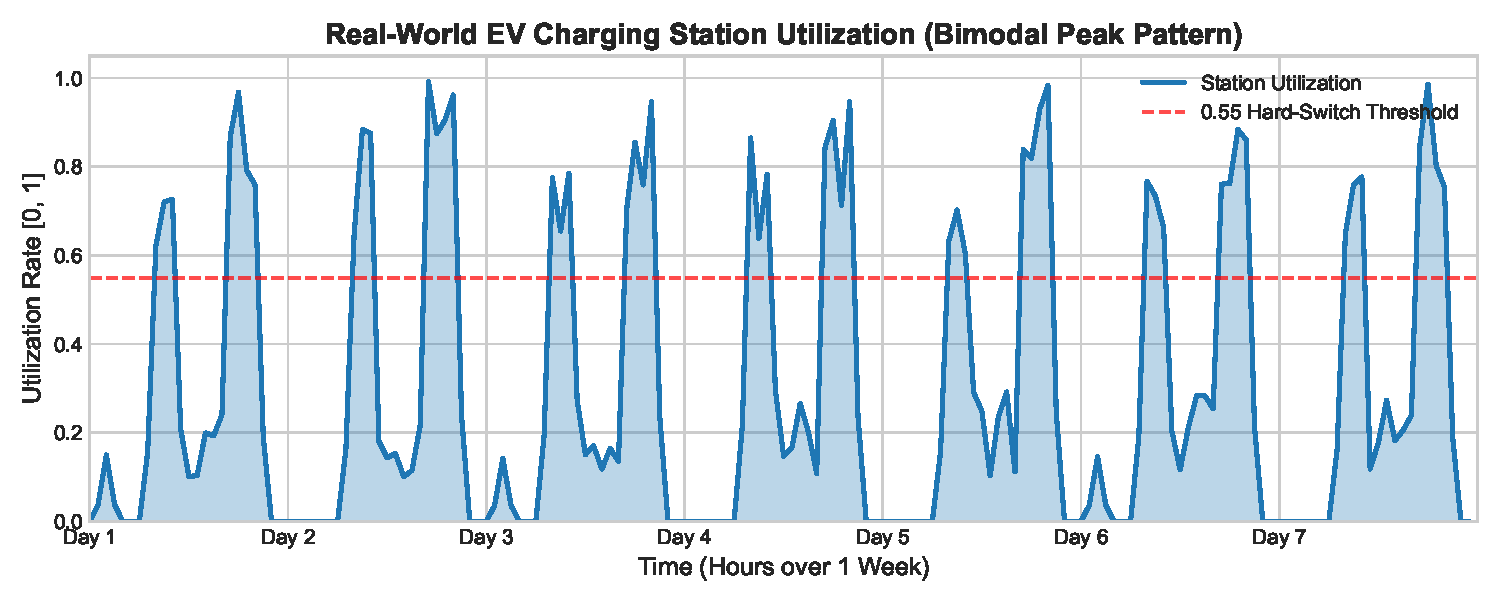
\includegraphics[width=0.9\textwidth]{images/eda_bimodal_peak.pdf}
\caption{Phân tích Dữ liệu Khám phá (EDA): Tỷ lệ sử dụng trạm sạc xe điện trong thế giới thực trong khoảng thời gian 1 tuần. Hình ảnh minh họa rõ ràng tính thưa thớt cực độ theo thời gian và biến động đỉnh lưỡng đỉnh, nơi mà các giai đoạn dài tỷ lệ sử dụng gần bằng không bị gián đoạn đột ngột bởi các đợt sạc tăng cao cục bộ.}\label{fig:eda_bimodal}
\end{figure}

Thách thức kép về tính thưa thớt cực độ và kích thước mẫu bị hạn chế này chi phối việc lựa chọn chiến lược các thuật toán dự báo. Tài liệu về dự báo phụ tải thường mặc định sử dụng các kiến trúc Học Sâu (Deep Learning), đặc biệt là mạng Bộ nhớ Ngắn Dài hạn (Long Short-Term Memory - LSTM), do khả năng vượt trội của chúng trong việc lập mô hình các phụ thuộc tuần tự. Tuy nhiên, các mạng nơ-ron sâu đòi hỏi lượng dữ liệu lớn và dễ bị quá khớp (overfitting) khi đối mặt với các tập dữ liệu quy mô nhỏ mang tính ngẫu nhiên. Chúng tối ưu hóa trên các đa tạp liên tục, nhiều chiều, do đó gặp khó khăn trong việc ánh xạ các bước nhảy rời rạc, không liên tục đặc trưng cho các đợt tăng vọt đột ngột của việc sạc xe điện.

Ngược lại, các mô hình kết hợp dựa trên cây (ensemble tree-based models)---đáng chú ý nhất là XGBoost, LightGBM và Random Forest---hoạt động trên một hệ hình toán học hoàn toàn khác, được điều chỉnh cho phù hợp với môi trường này. Các thuật toán dựa trên cây phân chia không gian đặc trưng sử dụng các phép tách trực giao, cứng nhắc, cấp cho chúng khả năng cô lập và ghi nhớ các bất thường rời rạc, tần số cao mà không ép buộc một mối quan hệ toán học liên tục trên toàn bộ đa tạp dữ liệu thưa thớt. Phép xấp xỉ hằng số từng mảng (piecewise constant approximation) này vượt trội trong các cấu trúc dữ liệu bảng nhỏ, vì cơ chế kết hợp làm chính quy hóa (regularizes) không gian dự đoán, giảm thiểu đặc tính quá khớp của các mô hình học sâu. Hơn nữa, framework gradient boosting lặp đi lặp lại việc ưu tiên giảm thiểu các phần dư tuần tự, làm cho nó trở nên lão luyện trong việc ánh xạ các bước nhảy rời rạc, phi tuyến vốn có của biến động đỉnh lưỡng đỉnh. Do đó, đối với miền hoạt động của dự báo phụ tải xe điện cục bộ, thưa thớt và bất thường này, các mô hình dữ liệu bảng dựa trên cây cung cấp một cơ sở mạnh mẽ và hợp lý so với các kiến trúc học sâu nguyên khối (monolithic deep learning frameworks).

Bất chấp sự vượt trội về kiến trúc của XGBoost và các mô hình dữ liệu bảng đối với dữ liệu thưa thớt, việc triển khai chúng ở cấu hình mặc định (out-of-the-box) dẫn đến hiệu suất thấp tại các đỉnh. Điều này xảy ra do hàm mục tiêu mặc định của chúng, điển hình là Sai số Toàn phương Trung bình (MSE), mang tính hướng tới giá trị trung bình (mean-seeking). Nó tối ưu hóa cho các thung lũng dày đặc, ổn định và bỏ qua các đỉnh cực đoan hiếm gặp, gây ra tình trạng dự báo thấp kinh niên. Hạn chế cơ bản này đòi hỏi một sự can thiệp vào không gian đầu ra, dẫn đến các chiến lược tối ưu hóa nâng cao được thảo luận tiếp theo.

\subsection{Phân tích Độ trễ và Lựa chọn Đặc trưng}\label{subsec:lag_analysis}
Trong nỗ lực tối ưu hóa các đầu vào của mô hình, việc đánh giá ban đầu về các phụ thuộc lịch sử là tối quan trọng. Hình~\ref{fig:acf_pacf} trình bày các biểu đồ Hàm Tự tương quan (ACF) và Hàm Tự tương quan Riêng phần (PACF), cho thấy rõ ràng các đỉnh tương quan nổi bật tại các độ trễ 1, 2, 4 và 24. Các độ trễ cụ thể này tóm gọn hiệu quả cả tính liên tục tức thời và tính chu kỳ ngày đêm 24 giờ vốn có trong nhu cầu sạc xe điện.

\begin{figure}[h]
\centering
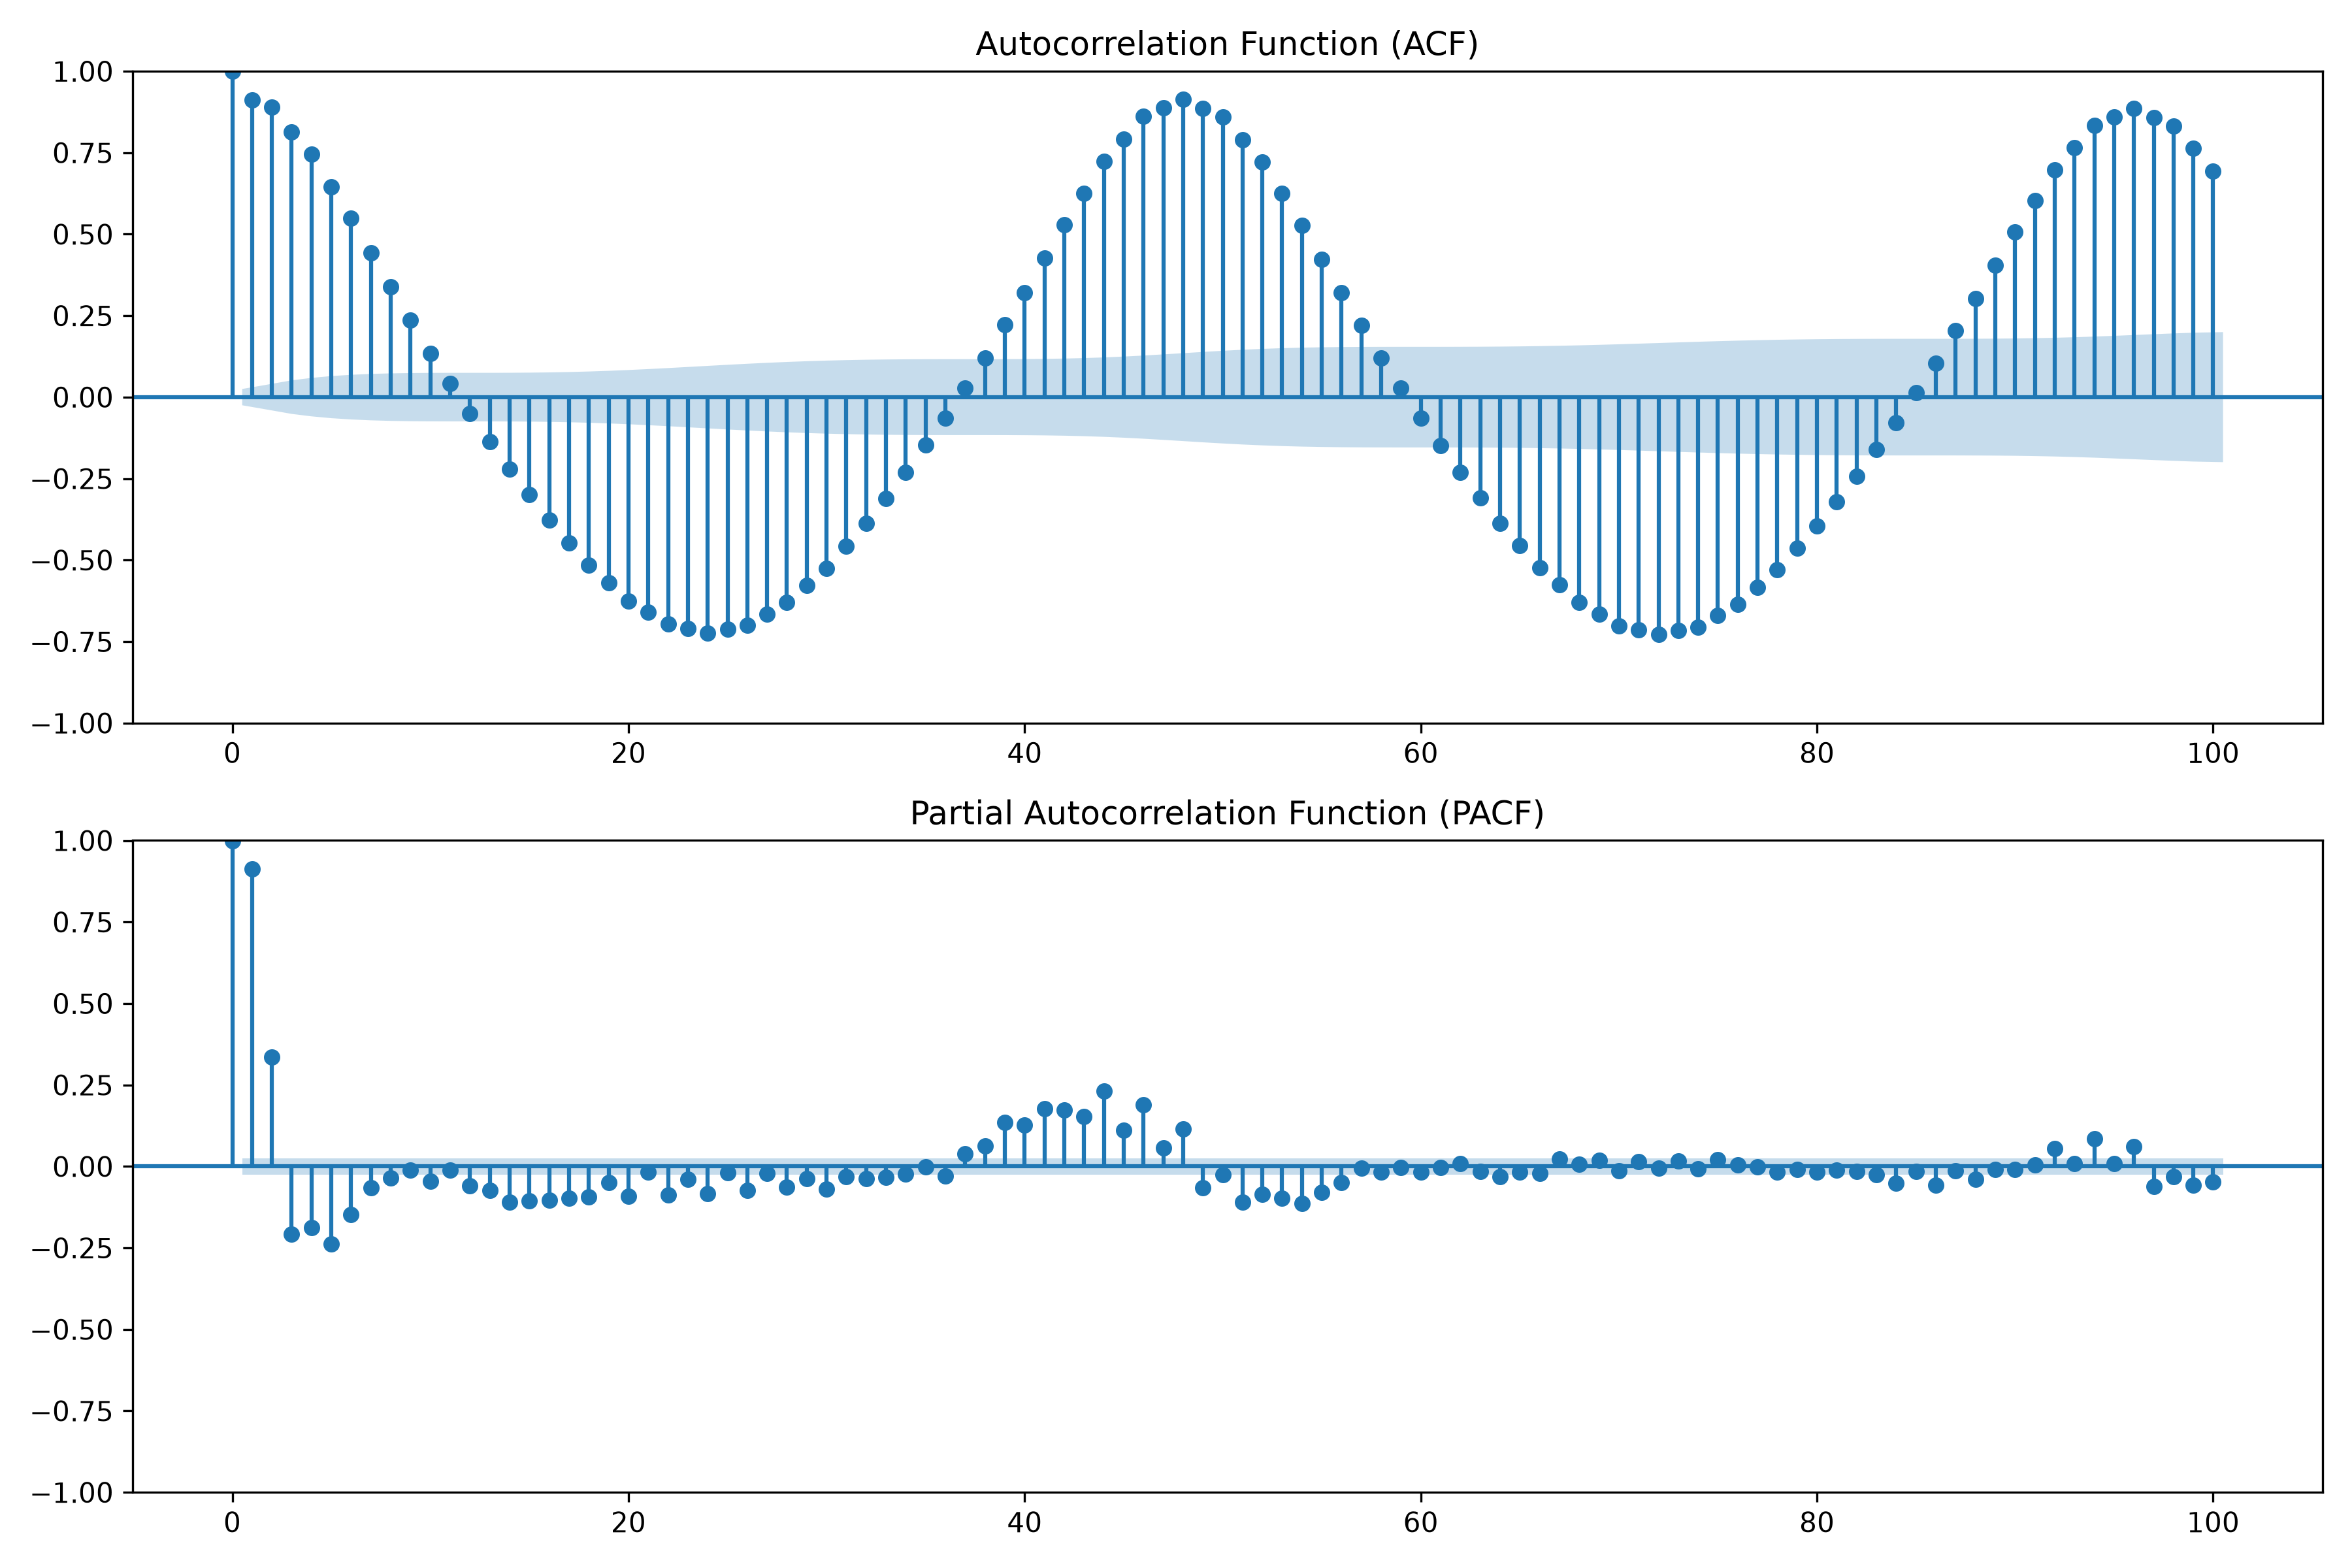
\includegraphics[width=0.8\textwidth]{images/acf_pacf.png}
\caption{Biểu đồ ACF và PACF minh họa các tương quan thời gian đáng kể tại các độ trễ mục tiêu.}\label{fig:acf_pacf}
\end{figure}

Để xác nhận chắc chắn việc lựa chọn các độ trễ này, một quá trình Tối ưu hóa siêu tham số (Hyper-Tuning) toàn diện đã được thực hiện sử dụng framework Optuna trên nhiều tổ hợp độ trễ khác nhau. Biểu hiện trực quan của quá trình tối ưu hóa này, được mô tả trong Hình~\ref{fig:lag_optimization}, chứng minh rằng tập con đặc trưng cụ thể bao gồm $\{1, 2, 4, 24\}$ đạt được hiệu suất chưa từng có, ghi nhận Sai số Toàn phương Trung bình (RMSE) và Sai số Tuyệt đối Trung bình (MAE) ở mức tối thiểu.

\begin{figure}[h]
\centering
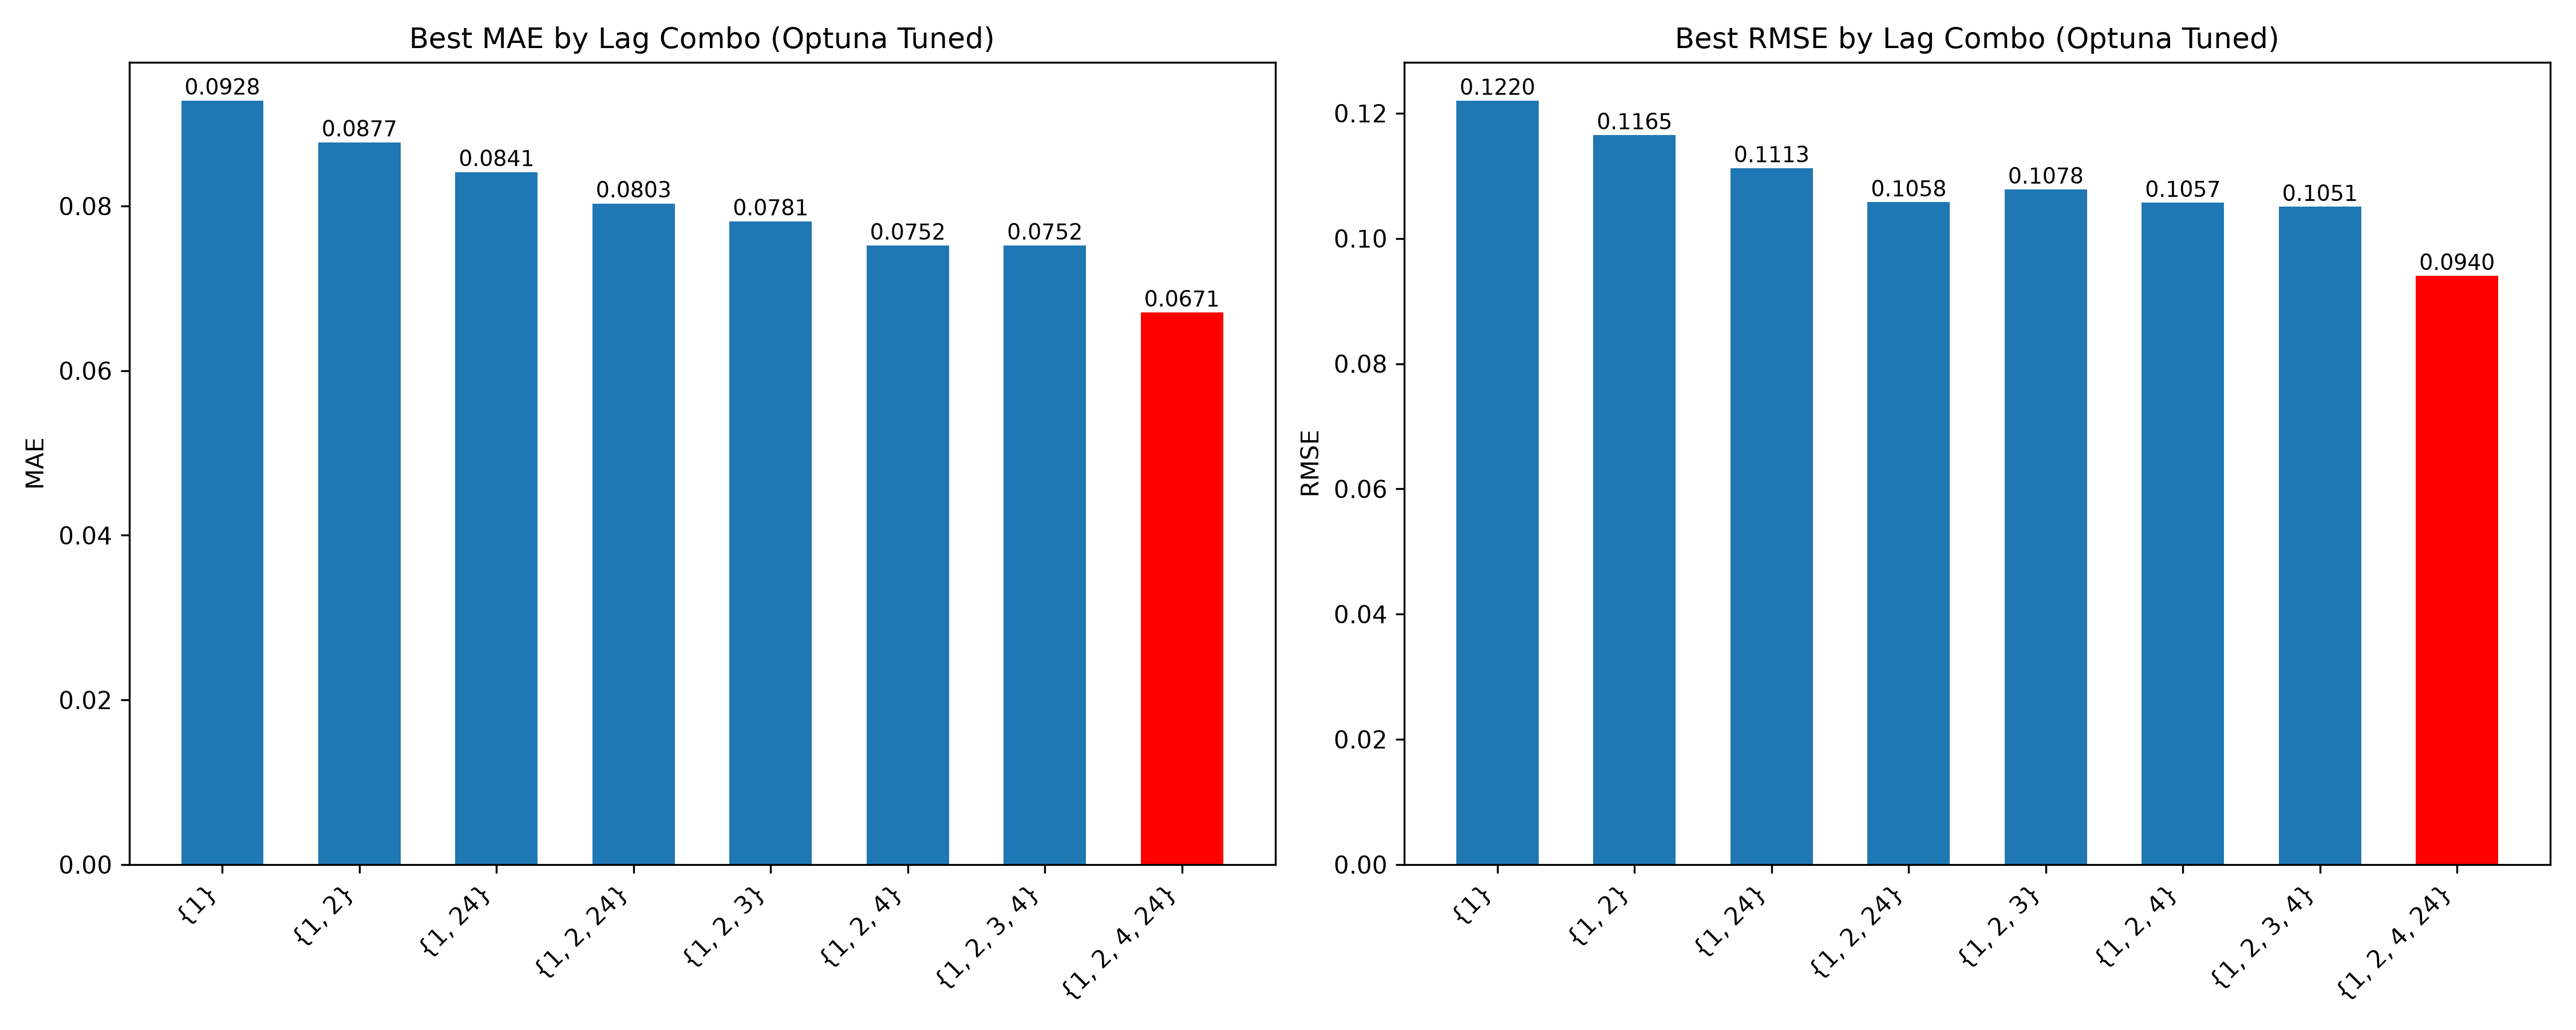
\includegraphics[width=0.8\textwidth]{images/lag_optimization.png}
\caption{Đánh giá hiệu suất của các tổ hợp độ trễ khác nhau thông qua Tối ưu hóa siêu tham số bằng Optuna, xác định $\{1, 2, 4, 24\}$ là tập hợp tối ưu.}\label{fig:lag_optimization}
\end{figure}

Hơn nữa, biểu đồ Độ quan trọng Đặc trưng của LightGBM (Hình~\ref{fig:feature_importance}) củng cố mạnh mẽ những phát hiện này. Bằng chứng thực nghiệm khẳng định một cách rõ ràng sự ưu việt tuyệt đối trong dự đoán của tập hợp biến độ trễ được chọn $\{1, 2, 4, 24\}$ khi so sánh với một loạt các biến ngoại sinh, chứng minh cho phương pháp luận trích xuất đặc trưng của chúng tôi và đảm bảo một vector đầu vào tinh gọn, hiệu suất cao.

\begin{figure}[h]
\centering
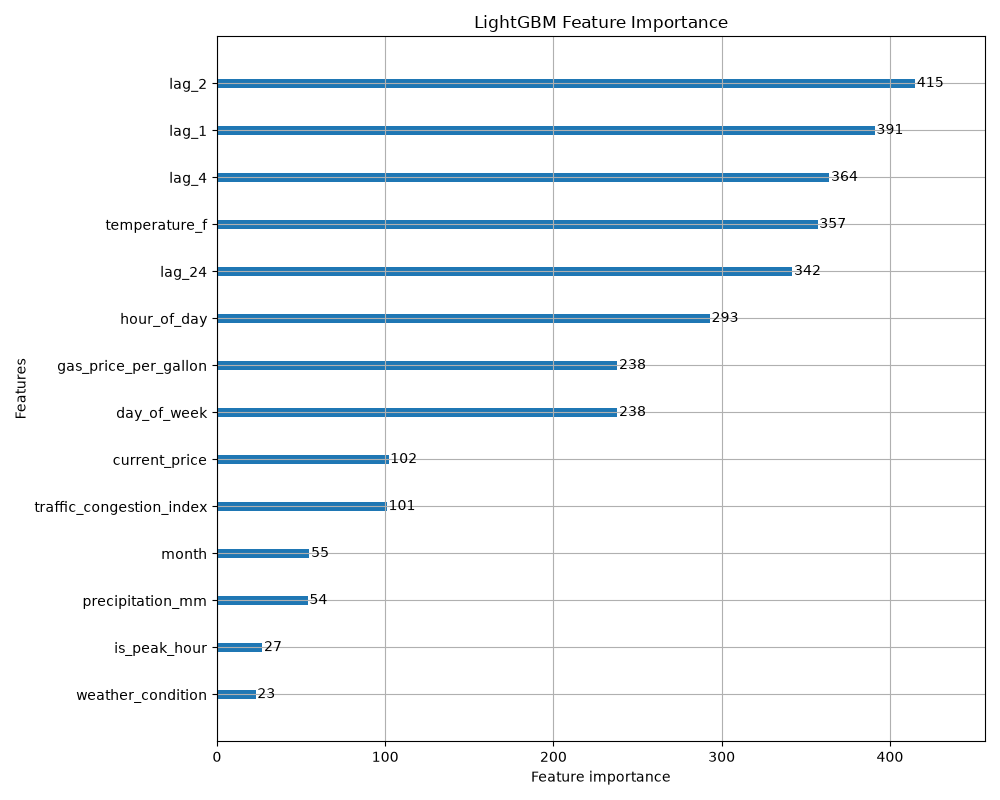
\includegraphics[width=0.8\textwidth]{images/feature_importance.png}
\caption{Độ quan trọng Đặc trưng của LightGBM củng cố sức mạnh dự đoán vượt trội của các biến độ trễ được chọn.}\label{fig:feature_importance}
\end{figure}

\subsection{Sự vượt trội của các mô hình dạng bảng so với Học sâu}\label{subsec3_1}
Để kiểm chứng thực nghiệm các luận điểm lý thuyết đã trình bày trong Mục \ref{subsec:data_characteristics}, một phân tích so sánh ban đầu đã được tiến hành nhằm đánh giá các mô hình dạng bảng dựa trên cây (tree-based tabular models) tiên tiến nhất so với một kiến trúc Học sâu (Deep Learning) tiêu biểu, cụ thể là mạng Bộ nhớ ngắn hạn dài (Long Short-Term Memory - LSTM). Thang đo đánh giá chính, Sai số toàn phương trung bình (Root Mean Squared Error - RMSE), được sử dụng để định lượng sai lệch dự báo tuyệt đối trong toàn bộ phạm vi dự báo cơ sở. Các kết quả thực nghiệm, được trình bày chi tiết và có hệ thống trong Bảng \ref{tab:rmse_comparison}, đã chứng minh một cách rõ ràng sự vượt trội hoàn toàn của các phương pháp học tập hợp dựa trên cây (ensemble tree-based) trong các điều kiện ràng buộc vận hành với dữ liệu cực kỳ thưa thớt và mức độ biến động cục bộ cao.

\begin{table}[h]
\caption{So sánh RMSE và MAE của các mô hình cơ sở trong việc dự báo Mức độ sử dụng trạm sạc EV}\label{tab:rmse_comparison}
\begin{tabular}{@{}lll@{}}
\toprule
Mô hình & RMSE & MAE \\
\midrule
Random Forest & 0.0769 & 0.0556 \\
XGBoost & 0.1085 & 0.0897 \\
LightGBM & 0.1503 & 0.1204 \\
LSTM (Học sâu) & 0.4216 & 0.3276 \\
\botrule
\end{tabular}
\end{table}

Các bằng chứng thực nghiệm đã bộc lộ rõ rệt sự thất bại hoàn toàn của mạng LSTM, khi cho ra giá trị RMSE cực kỳ cao ở mức 0.4216. Sự sụt giảm hiệu suất nghiêm trọng này củng cố trực tiếp cho giả thuyết lý thuyết trước đó của chúng tôi: các mạng nơ-ron sâu nguyên khối (monolithic), vốn chủ yếu tối ưu hóa trên các đa tạp khả vi (differentiable manifolds) đa chiều và liên tục, có cấu trúc không phù hợp để ánh xạ các bước nhảy đỉnh (peak jumps) hai mốt rời rạc và gián đoạn cao - một đặc trưng của các đợt tăng vọt đột ngột trong nhu cầu sạc EV. Khi bị giới hạn bởi kích thước mẫu nhỏ đặc trưng của dữ liệu cấp trạm sạc, mạng LSTM chắc chắn sẽ cố gắng thiết lập một mối quan hệ liên tục mượt mà xuyên qua sự thưa thớt về mặt thời gian đầy biến động này, dẫn đến hiện tượng làm mịn quá mức (over-smoothing) nghiêm trọng và hoàn toàn mất đi khả năng nắm bắt các cú sốc cục bộ tần số cao.

Ngược lại, các mô hình tập hợp dựa trên cây lại thể hiện tính bền vững về mặt toán học và độ chính xác dự báo đặc biệt xuất sắc. Random Forest đạt mức RMSE cơ sở rất cạnh tranh là 0.0769, tiếp theo là XGBoost với 0.1085 và LightGBM với 0.1503. Những chỉ số này đã chứng thực một cách mạnh mẽ tiền đề cho rằng các thuật toán dạng bảng - vốn sử dụng các phân chia trực giao (orthogonal splits) cứng nhắc để phân hoạch không gian đặc trưng - được thiết kế đặc biệt phù hợp cho môi trường phức tạp này. Khả năng vốn có của chúng trong việc xấp xỉ hằng số từng mảng (piecewise constant approximation) cho phép chúng phân lập và ánh xạ các đỉnh bất thường rời rạc một cách liền mạch mà không gây ra những sai lệch toán học liên tục trong các trạng thái đáy (valley states) ổn định. Bằng cách giảm thiểu về bản chất các điểm yếu dễ bị quá khớp (overfitting) nghiêm trọng thường ảnh hưởng đến các mạng nơ-ron ngốn dữ liệu trên các tập dữ liệu nhỏ, các mô hình dựa trên cây đã thiết lập một cách chắc chắn một nền tảng toán học vững chắc để dự báo các phụ tải sạc EV biến động bất thường.

\subsection{Hiệu suất của toán học bắt đỉnh và kiến trúc hai giai đoạn}\label{subsec3_2}

Những hạn chế cốt lõi của các kỹ thuật hồi quy tiêu chuẩn trở nên đặc biệt rõ rệt khi dự báo các sự kiện sạc ở mức cực đoan. Như được minh họa trong Hình \ref{fig:base_model}, Mô hình cơ sở (Baseline Model), được tối ưu hóa thông qua Sai số toàn phương trung bình (MSE) tiêu chuẩn, liên tục dự báo dưới mức (under-forecast) đối với các đỉnh sạc phi tuyến. Vì hàm mục tiêu MSE về mặt toán học mang tính chất "tìm kiếm giá trị trung bình" (mean-seeking), nó ưu tiên rất mạnh cho các vùng đáy (valleys) thấp điểm dày đặc và ổn định, trong khi phần lớn bỏ qua các sự kiện cực đoan thưa thớt, dẫn đến một phản hồi dự báo đỉnh có thể đoán trước được nhưng lại cực kỳ thiếu chính xác.

\begin{figure}[h]
    \centering
    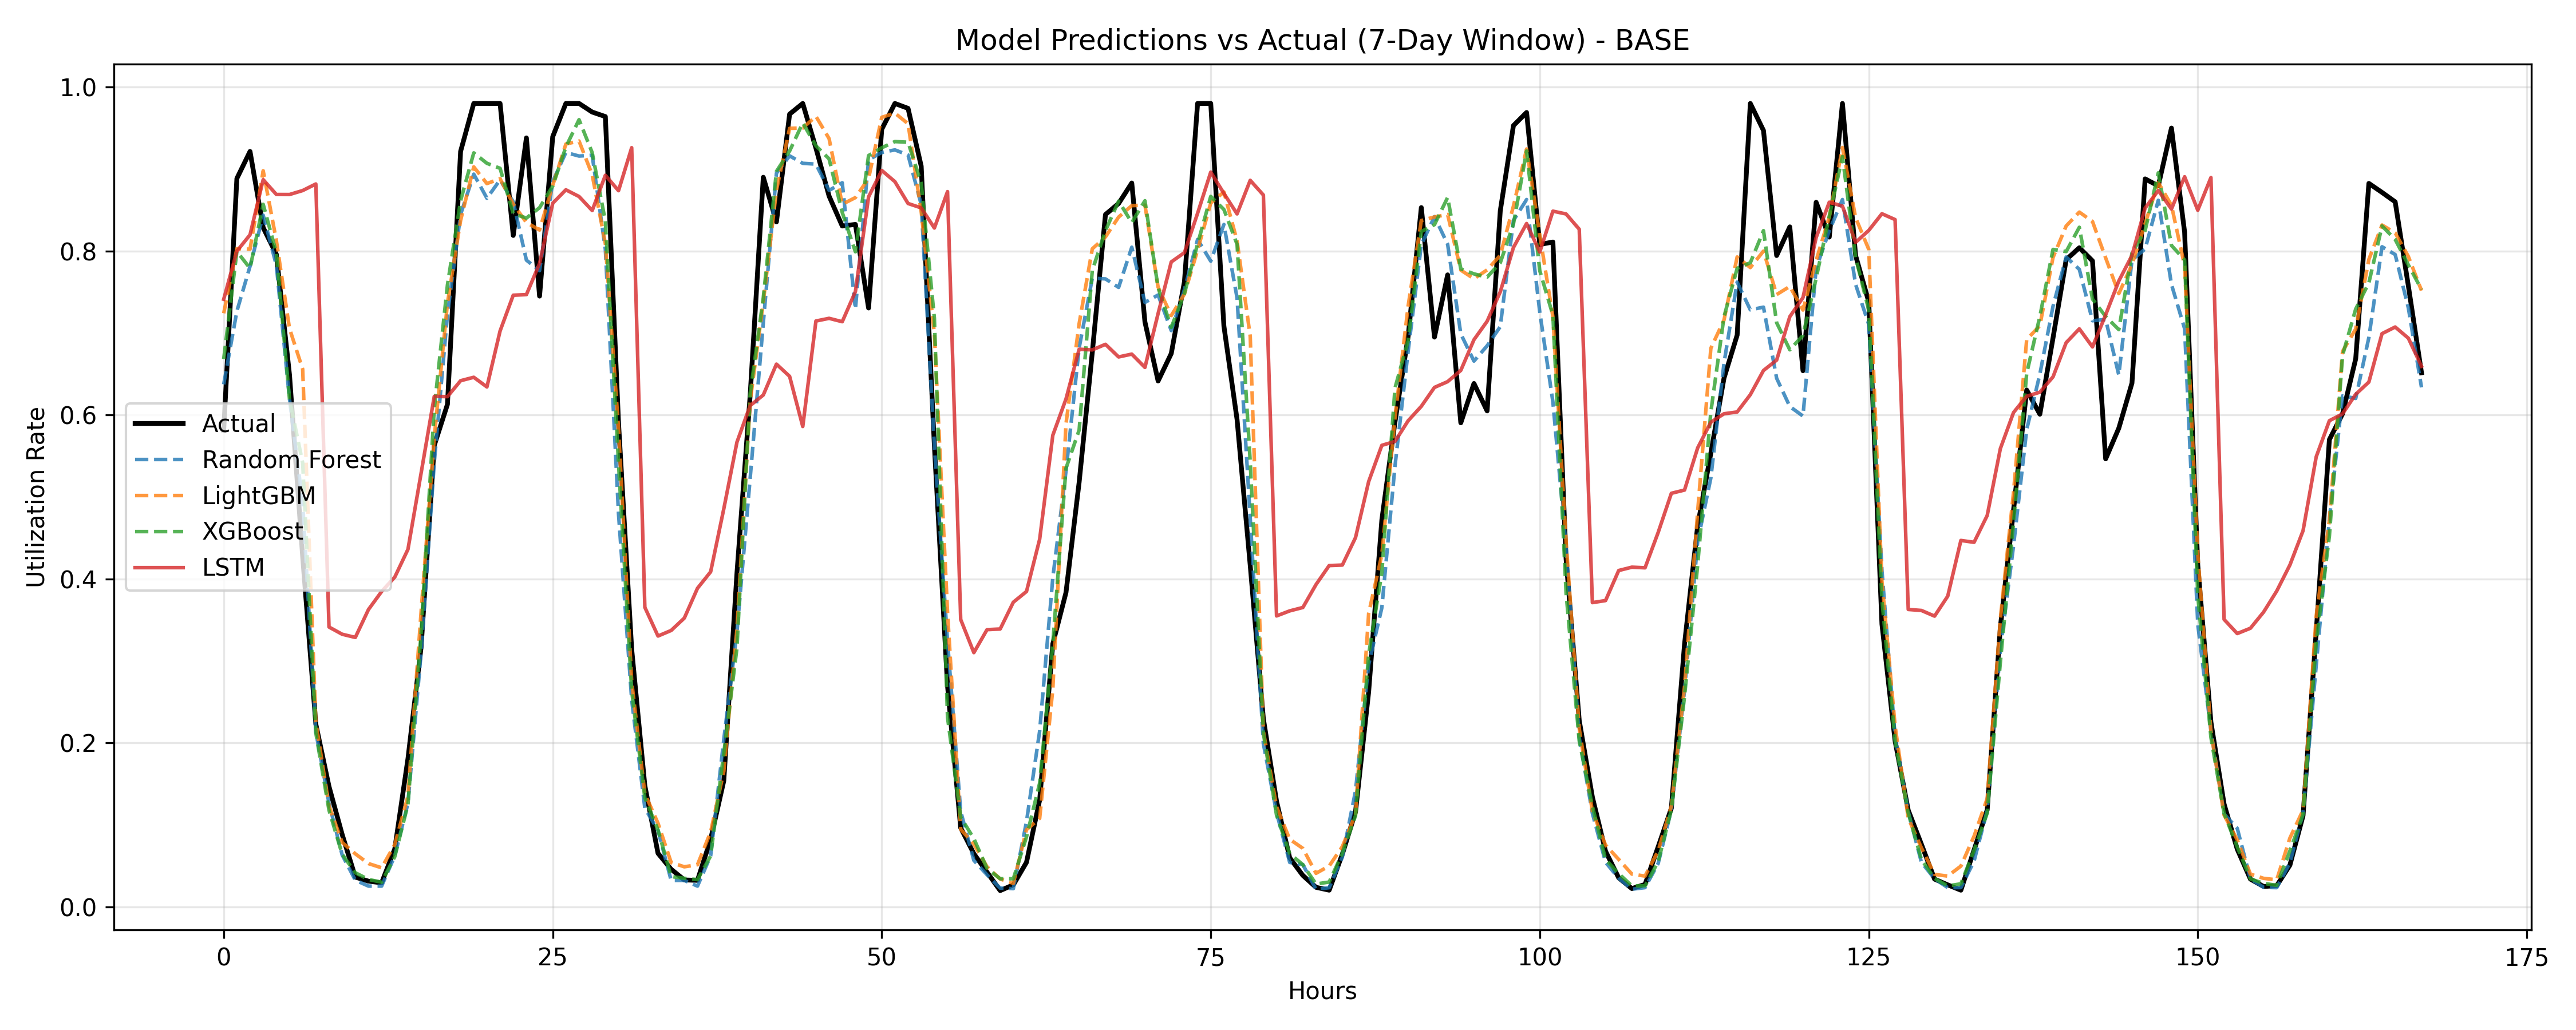
\includegraphics[width=0.9\textwidth]{../workspace/figures/base_7days.png}
    \caption{Hiệu suất của Mô hình cơ sở (MSE), minh họa tình trạng dự báo dưới mức kinh niên đối với các đỉnh sạc EV cực đoan.}
    \label{fig:base_model}
\end{figure}

Để bắt buộc thuật toán tập trung lại vào những sự kiện quan trọng này mà không làm hỏng không gian phân phối đầu vào thông qua các kỹ thuật lấy mẫu tăng cường nhân tạo (synthetic oversampling), Phép biến đổi mục tiêu lũy thừa (Target Power Transformation - TPT, $y^3$) và Hàm mất mát bắt đỉnh tùy chỉnh (Custom Peak Loss) đã được tích hợp. Sự can thiệp toán học này tiến hành phạt nặng (aggressively penalize) các sai số biên độ lớn một cách có chủ đích tại các giới hạn trên cực đoan của phân phối mức độ sử dụng. Hình \ref{fig:tpt_model} minh họa sống động tác động sâu sắc của chiến lược này: Mô hình TPT đã nắm bắt thành công và quyết liệt các "đỉnh hai mốt" cực đoan mà Mô hình cơ sở đã thất bại trong việc dự báo. Tuy nhiên, sự tăng cường độ nhạy toán học này lại gây ra một hệ quả phụ nghiêm trọng. Việc bắt buộc các cây tăng cường độ dốc (gradient boosting trees) ưu tiên cho động học hỗn loạn của các đỉnh đã làm suy giảm tính toàn vẹn cấu trúc của mô hình trong các vùng đáy phẳng, ổn định, dẫn đến các dự báo thấp điểm có mức độ biến động và nhiễu rất cao.

\begin{figure}[h]
    \centering
    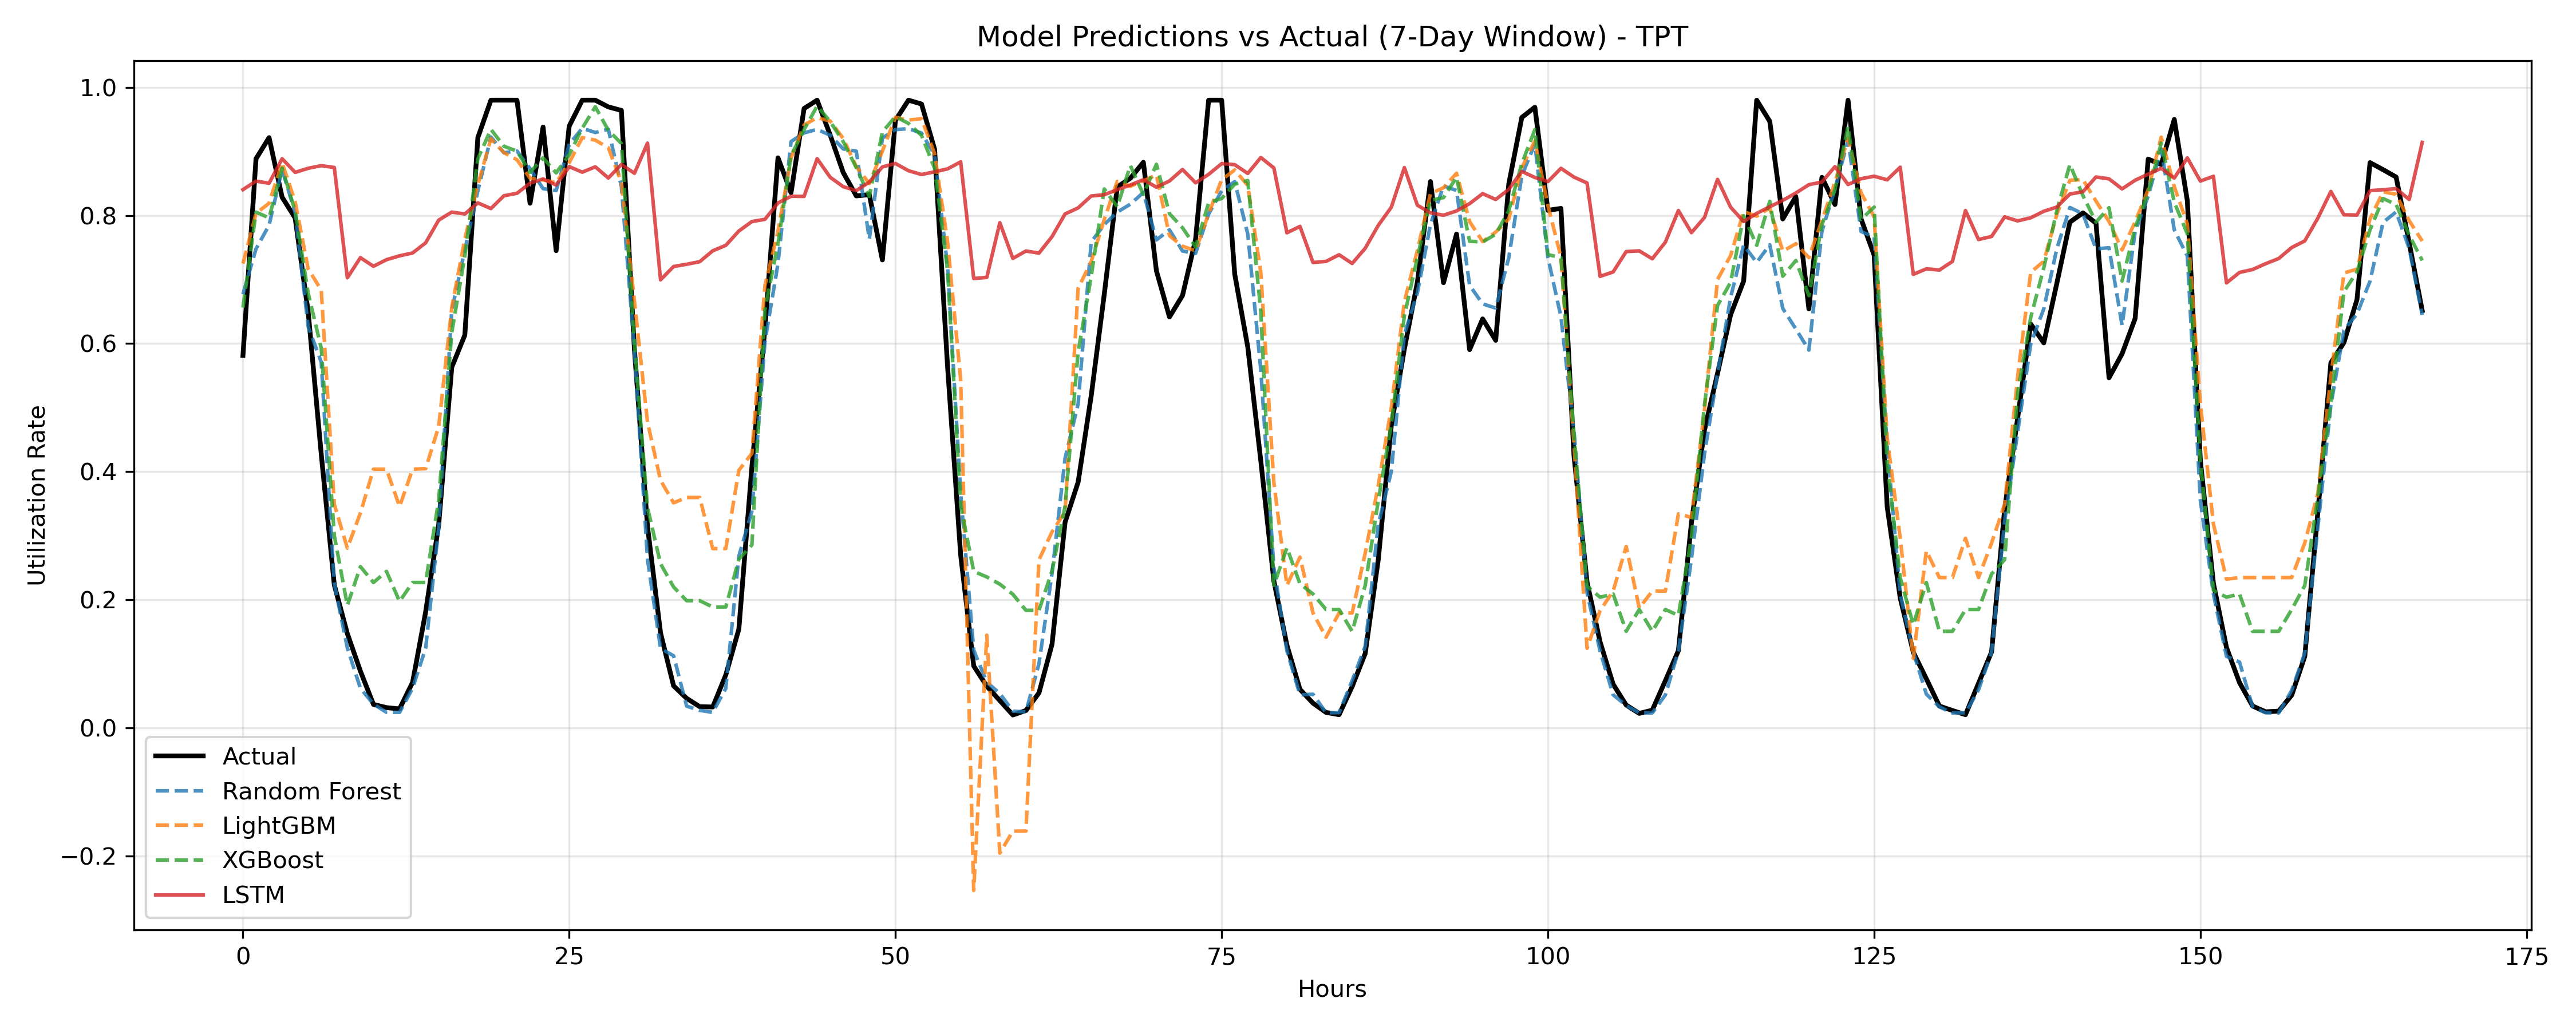
\includegraphics[width=0.9\textwidth]{../workspace/figures/tpt_7days.png}
    \caption{Hiệu suất của Mô hình TPT, làm nổi bật khả năng bắt đỉnh thành công nhưng độ ổn định ở vùng đáy lại bị suy giảm nghiêm trọng và nhiều nhiễu.}
    \label{fig:tpt_model}
\end{figure}

Sự đánh đổi phức tạp này về mặt toán học đòi hỏi một sự phân nhánh cấu trúc (structural bifurcation), dẫn đến Kiến trúc dựa trên quy tắc hai giai đoạn (Two-Stage Rule-Based Architecture) được chúng tôi đề xuất. Như được minh họa một cách rõ ràng trong Hình \ref{fig:two_stage_model}, cơ chế chuyển đổi theo quy tắc hai giai đoạn này đã dung hòa hoàn hảo các yêu cầu kép của hệ thống. Cụ thể, khi quỹ đạo cơ sở vượt qua ngưỡng $0.55$ được xác định chặt chẽ, hệ thống thực hiện chuyển đổi cứng (hard switch) sang dự báo TPT chủ động. Điều này vừa bảo vệ thành công các vùng đáy thấp điểm dày đặc khỏi sự biến động ngẫu nhiên, vừa nắm bắt hoàn hảo các đỉnh hai mốt sắc nhọn, đạt được một đường bao dự báo (predictive envelope) tối ưu toàn cục mà không cần đến sự phức tạp không cần thiết của mô hình phân loại.

\begin{figure}[h]
    \centering
    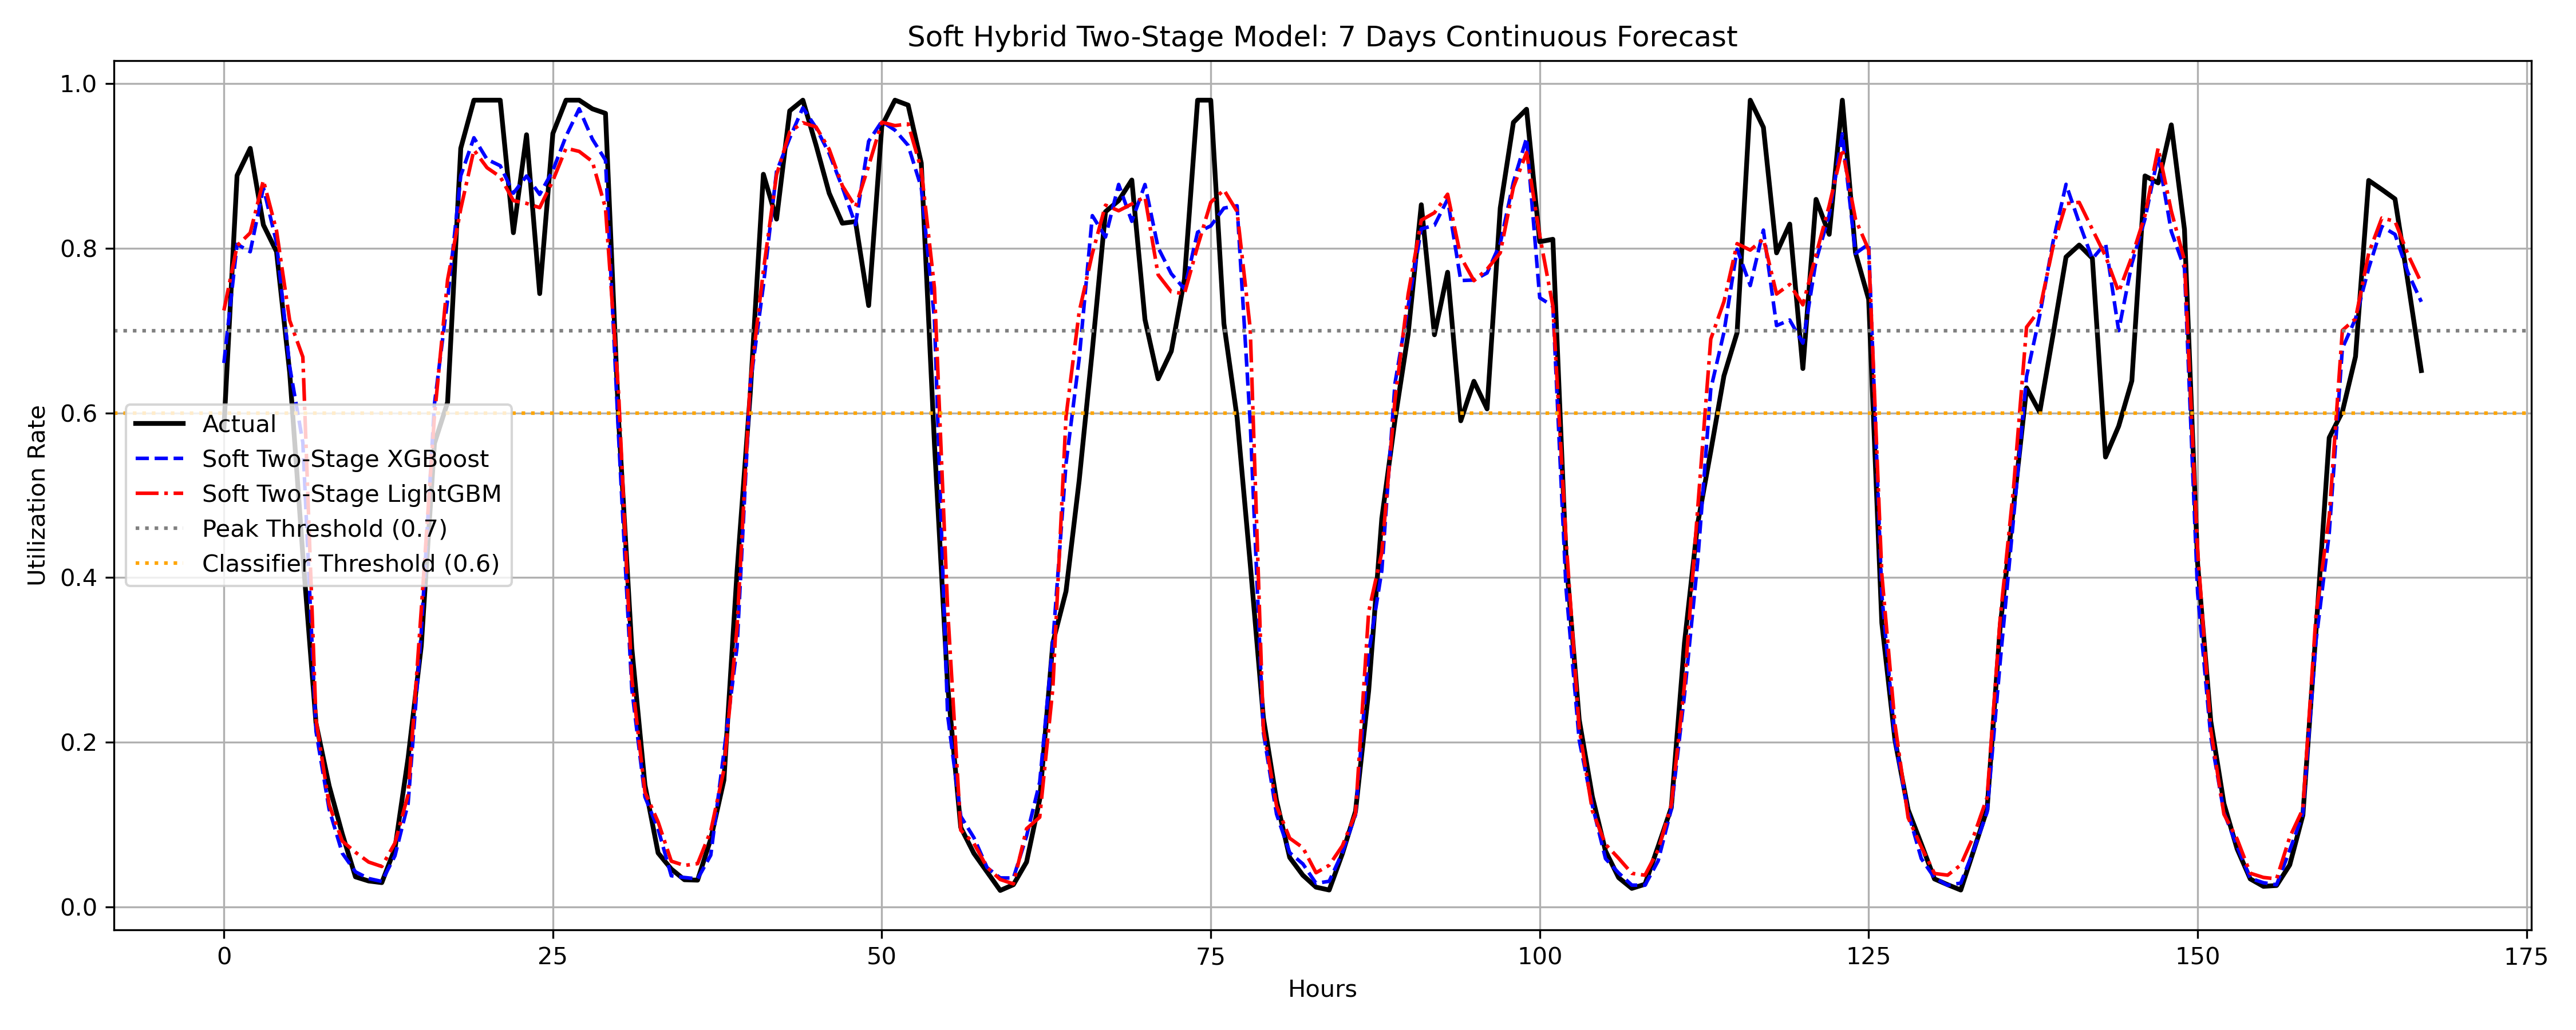
\includegraphics[width=0.9\textwidth]{../workspace/figures/two_stage_7days.png}
    \caption{Hiệu suất của Kiến trúc dựa trên quy tắc hai giai đoạn, dung hòa hoàn hảo giữa việc bảo vệ tính ổn định của vùng đáy và khả năng bắt đỉnh quyết liệt.}
    \label{fig:two_stage_model}
\end{figure}

\subsection{Phá vỡ độ trễ pha bằng tích hợp độ trễ biến đại diện (Proxy-Lag Integration)}\label{subsec3_3}
Một thách thức kéo dài trong bài toán dự báo phụ tải cực ngắn (dự báo trước 1 giờ) là hiện tượng "Độ trễ pha" (Phase Lag). Khi đối mặt với mức độ biến động tần số cao, các mô hình tự hồi quy tiêu chuẩn (ngay cả những mô hình được tăng cường với các Điểm chuyển trạng thái và các đặc trưng động học) có xu hướng toán học mặc định dự báo rằng giờ tiếp theo sẽ chỉ đơn thuần phản chiếu giờ trước đó. Hành vi trung bình hóa mang tính phòng thủ này dẫn đến một đường cong dự báo bị dịch chuyển hoặc trễ rõ rệt so với đường cong phụ tải thực tế, liên tục bỏ lỡ các đợt tăng hoặc giảm đột ngột như được minh họa trong Hình~\ref{fig:1h_phase_lag}.

\begin{figure}[h]
    \centering
    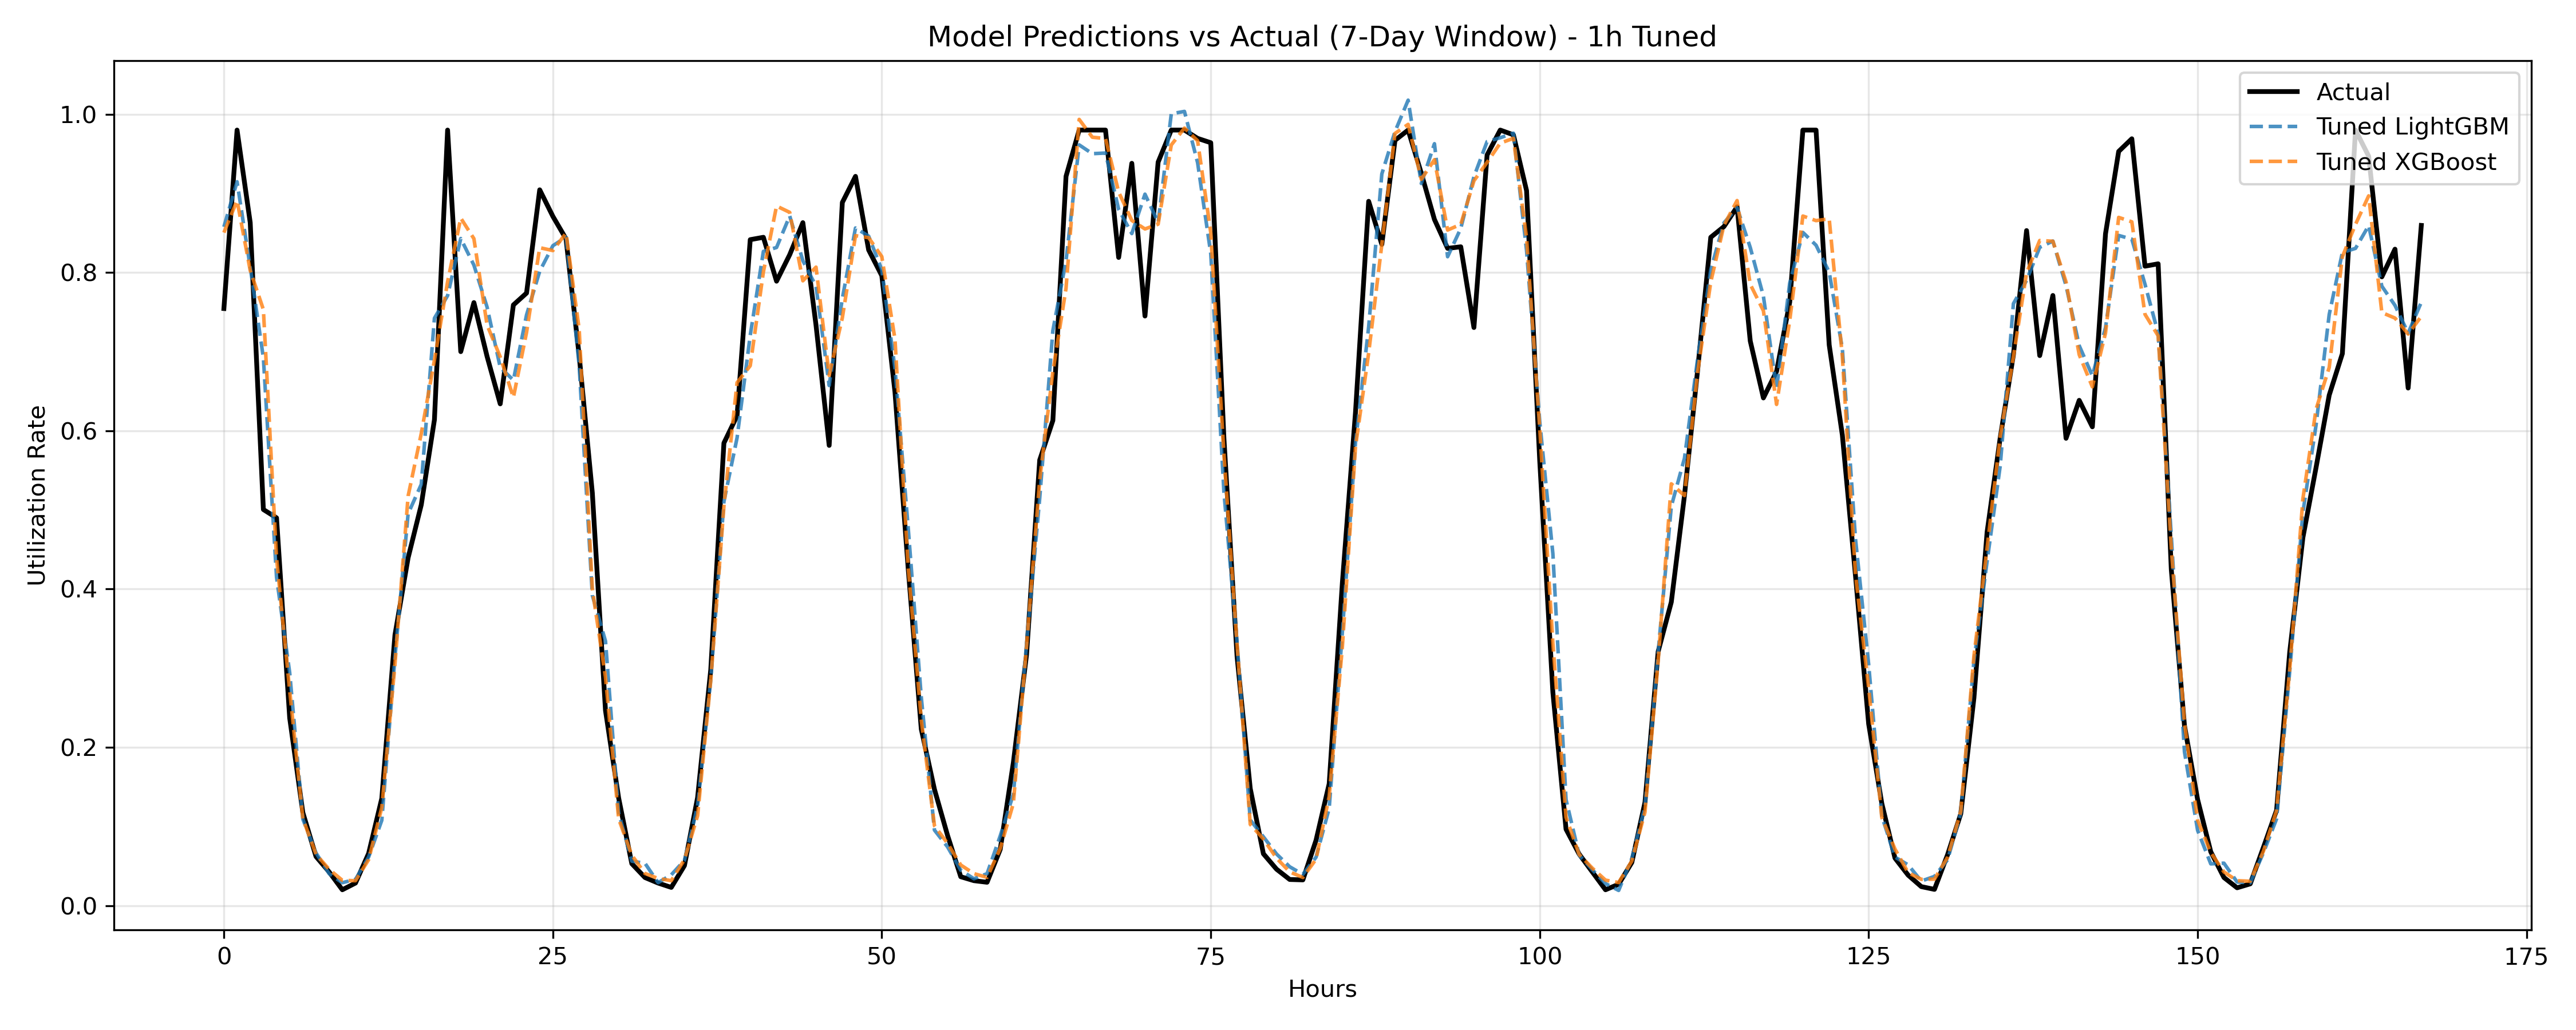
\includegraphics[width=0.9\textwidth]{../workspace/figures/1h_tune_7days.png}
    \caption{Mô hình dự báo 1 giờ tiêu chuẩn cho thấy hiện tượng Độ trễ pha cổ điển, trong đó các dự báo bị trễ đáng kể trong các đợt biến động phụ tải đột ngột.}
    \label{fig:1h_phase_lag}
\end{figure}

Để vượt qua hạn chế toán học cố hữu này, chúng tôi giới thiệu một bước đột phá về cấu trúc là Tăng cường đặc trưng đại diện (Proxy Feature Boosting). Thay vì loại bỏ bối cảnh thay đổi trong ngày (diurnal context), chúng tôi tích hợp trực tiếp quỹ đạo cơ sở chu kỳ 24 giờ như một đặc trưng chính. Bằng cách buộc mô hình dự báo mục tiêu tuyệt đối thông qua việc sử dụng biến đại diện này, độ trễ pha bị phá vỡ một cách hiệu quả. Mô hình được neo giữ bởi chu kỳ vĩ mô (macro-cycle) và có thể dành toàn bộ khả năng biểu diễn của nó cho việc dự báo các sai lệch tần số cao (Hình~\ref{fig:1h_residual}).

\begin{figure}[h]
    \centering
    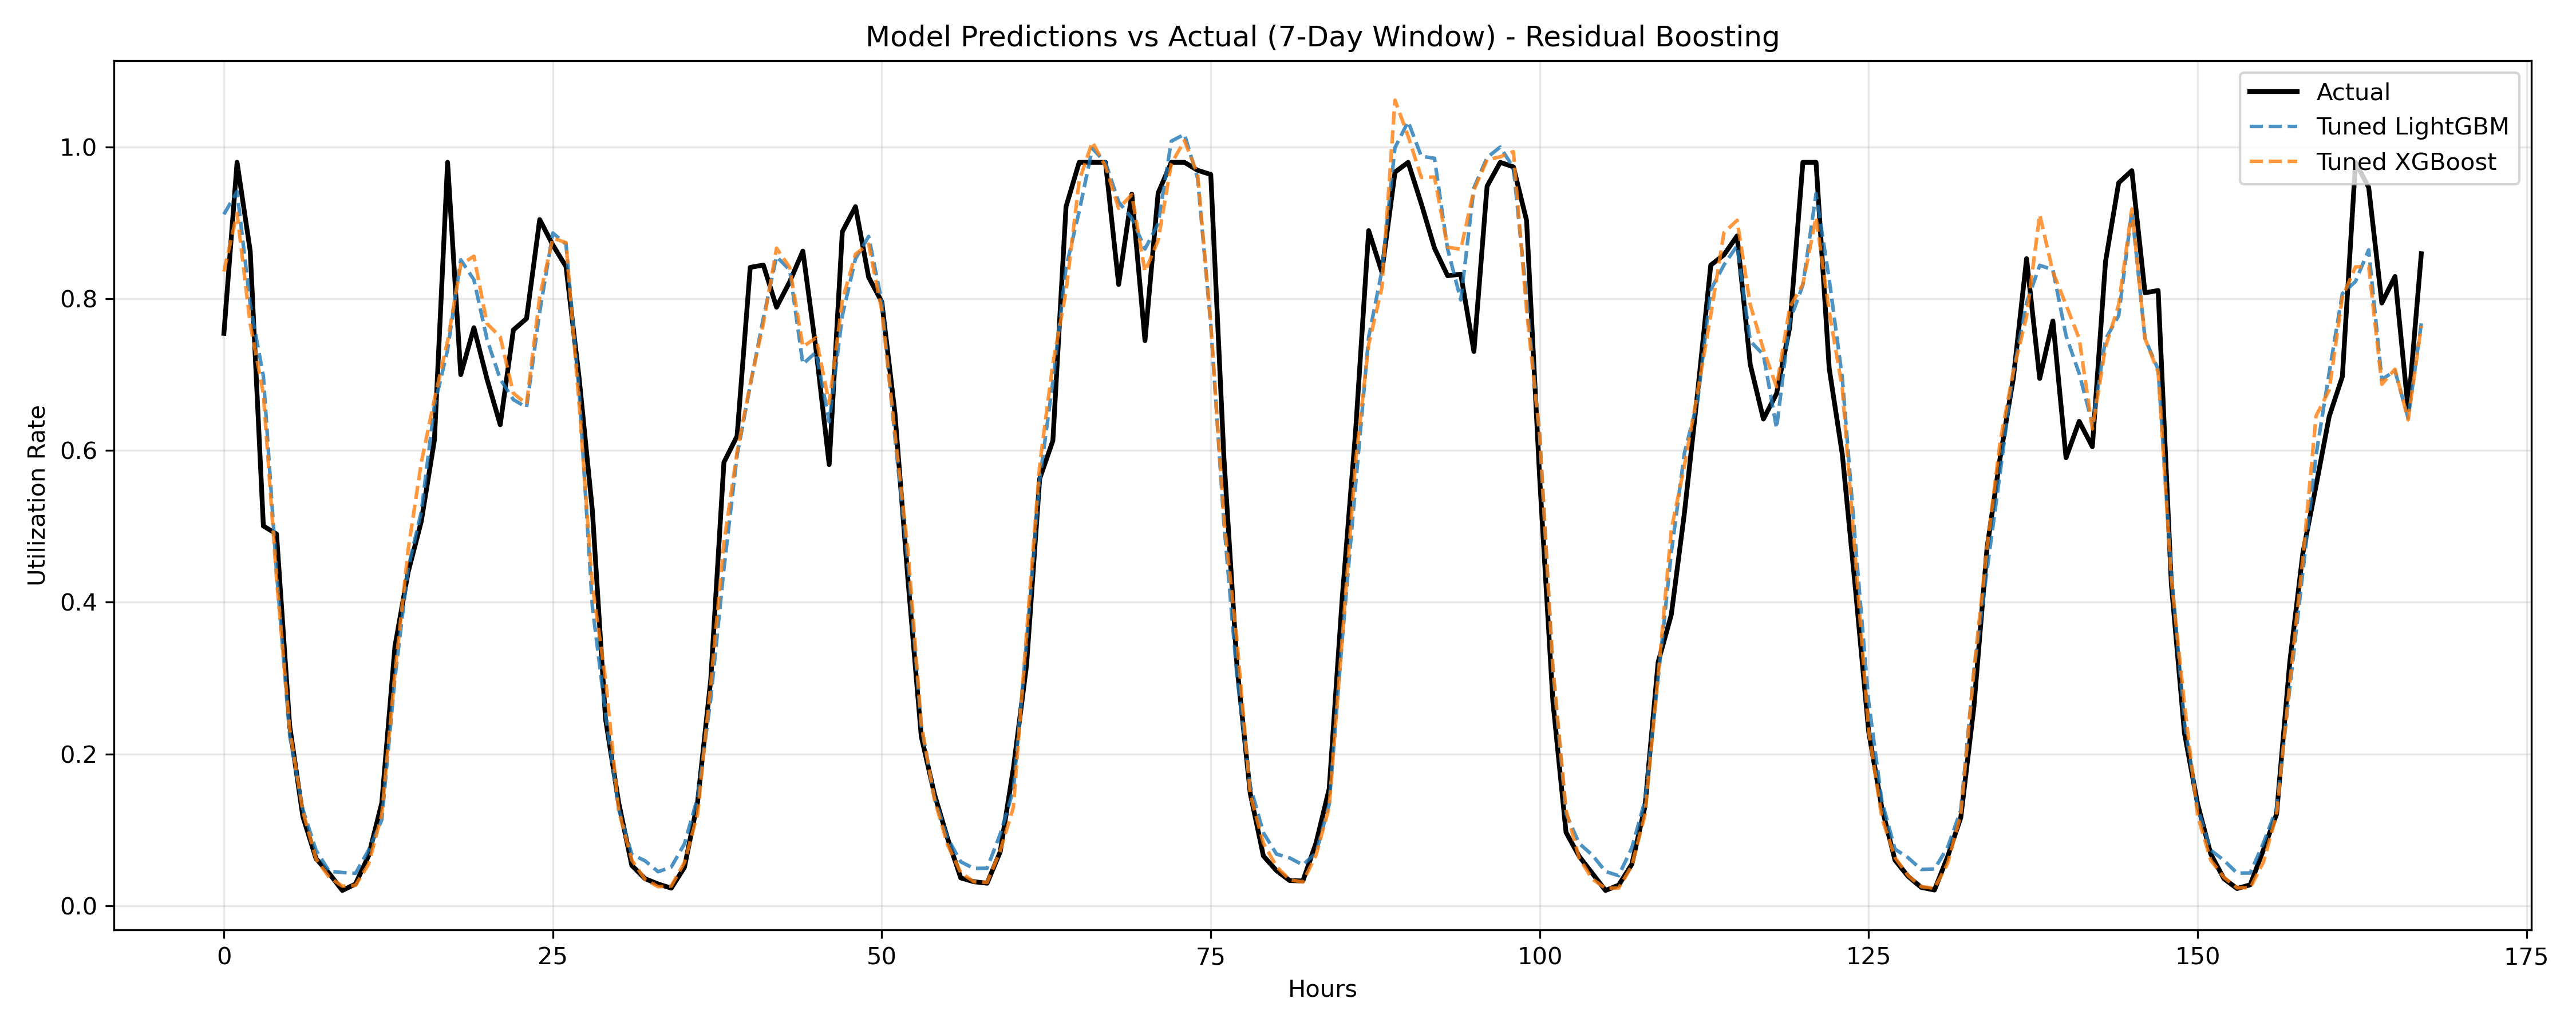
\includegraphics[width=0.9\textwidth]{../workspace/figures/1h_tune_residual_7days.png}
    \caption{Hiệu suất của Mô hình tinh chỉnh vi mô (Micro-Tuner). Bằng cách tích hợp đặc trưng đại diện, mô hình đã thoát khỏi độ trễ pha.}
    \label{fig:1h_residual}
\end{figure}

Cuối cùng, khái niệm này được hiện thực hóa hoàn toàn trong kiến trúc Chuỗi thác đại diện-độ trễ (Proxy-Lag Cascade). Trong cấu hình tối ưu này, quỹ đạo 24 giờ vĩ mô được cung cấp dưới dạng cấu trúc tiên nghiệm (structured prior) vào Mô hình tinh chỉnh vi mô 1 giờ. Sự kết hợp này tạo ra một hệ thống được tích hợp sâu sắc, sở hữu cả bộ nhớ chu kỳ dài hạn lẫn sự linh hoạt của phản xạ vi mô (microscopic reflex agility). Chuỗi thác đại diện-độ trễ đã loại bỏ hoàn toàn độ trễ pha, bám sát các điểm rẽ một cách tức thì và mang lại độ chính xác chưa từng có trên tất cả các thang thời gian (Hình~\ref{fig:proxy_cascade}).

\begin{figure}[h]
    \centering
    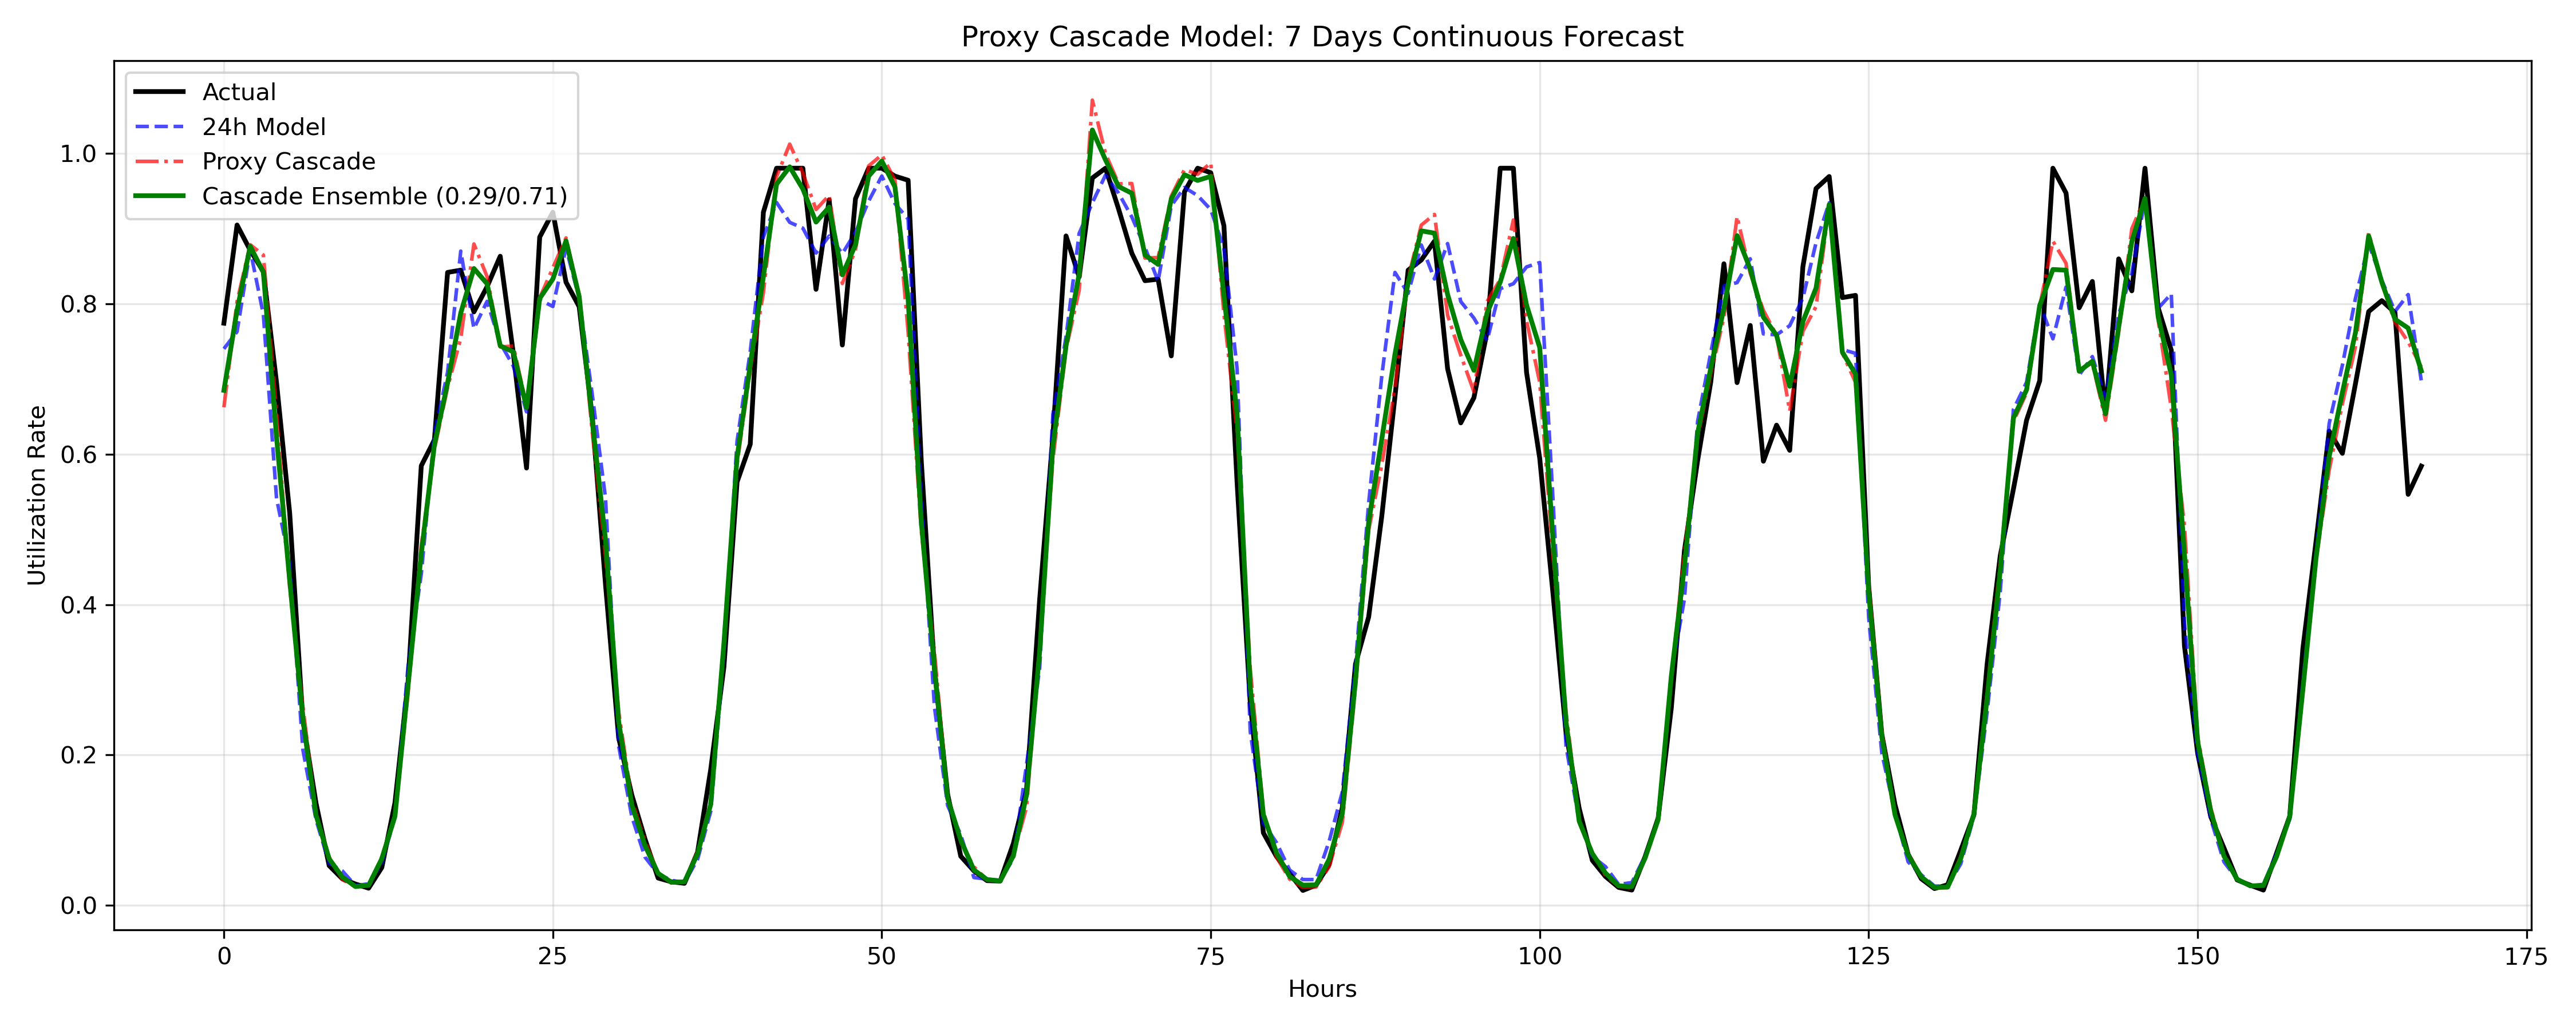
\includegraphics[width=0.9\textwidth]{../workspace/figures/proxy_cascade_7days.png}
    \caption{Kiến trúc Chuỗi thác đại diện-độ trễ (Proxy-Lag Cascade) hoàn chỉnh. Việc kết hợp bộ nhớ chu kỳ với sự linh hoạt của phản xạ vi mô đã loại bỏ hoàn toàn độ trễ pha và bám sát hoàn hảo các biến động đột ngột.}
    \label{fig:proxy_cascade}
\end{figure}

\subsection{Hiệu suất đột phá (State-of-the-Art) và Thảo luận về triển khai}\label{subsec3_4}

Sự tiến hóa trong kiến trúc được phát triển trong nghiên cứu này đã đạt đến đỉnh cao với Mô hình tập hợp Chuỗi thác đại diện-độ trễ (Proxy-Lag Cascade Ensemble), thiết lập một chuẩn mực mới trong dự báo mức độ sử dụng trạm sạc EV. Bảng \ref{tab:sota_rmse} tóm tắt sự phát triển theo thời gian của các mô hình của chúng tôi cùng với các chỉ số Sai số toàn phương trung bình (RMSE) tương ứng.

\begin{table}[h]
\caption{Quá trình phát triển các kiến trúc dự báo và Hiệu suất SOTA (Tiên tiến nhất) cuối cùng}\label{tab:sota_rmse}
\begin{tabular}{@{}lll@{}}
\toprule
Kiến trúc & RMSE & MAE \\
\midrule
Mô hình cơ sở XGBoost (24h) & 0.1085 & 0.0897 \\
Kiến trúc hai giai đoạn dựa trên quy tắc (24h) & 0.0753 & 0.0524 \\
Chuỗi thác đại diện-độ trễ hoàn chỉnh (24h + 1h) & \textbf{0.0664} & \textbf{0.0456} \\
\botrule
\end{tabular}
\end{table}

Mô hình cơ sở XGBoost, mặc dù mạnh mẽ, vẫn mang lại mức RMSE là 0.1085 do thiếu khả năng cân bằng đồng thời giữa các vùng đáy thấp điểm dày đặc và các đỉnh cực đoan thưa thớt. Việc ứng dụng kiến trúc hai giai đoạn dựa trên quy tắc đã giải quyết thành công mâu thuẫn này, giúp giảm đáng kể sai số xuống còn 0.0753. Cuối cùng, sự tích hợp của Mô hình tinh chỉnh vi mô 1 giờ vào trong kiến trúc Chuỗi thác đại diện-độ trễ đã xóa bỏ hoàn toàn hiện tượng trễ pha theo thời gian, đạt được mức RMSE tiên tiến nhất (SOTA) là 0.0664. Tiến trình này đã chứng minh rõ ràng tính cấp thiết của mô hình thiết kế phân cấp mà chúng tôi đề xuất.

Một thành phần then chốt của kiến trúc hoàn chỉnh này là "Tỷ lệ Vàng" (Golden Ratio) được đúc kết từ thực nghiệm nhằm điều phối sự tổng hợp giữa hai tầm nhìn vĩ mô và vi mô: $\hat{y}_{final} = 0.33 \times \hat{y}_{24h} + 0.67 \times \hat{y}_{1h\_micro}$. Ý nghĩa toán học của tỷ lệ này nằm ở khả năng dung hòa hoàn hảo các động lực thời gian. Việc phân bổ $1/3$ trọng số dự báo cho biến đại diện 24 giờ sẽ cung cấp "lực hấp dẫn chu kỳ" (cyclical gravity) thiết yếu, đảm bảo rằng mô hình vẫn bám chặt vào quỹ đạo cơ sở trong ngày và ngăn chặn các ảo giác thuật toán (algorithmic hallucinations) trong các chu kỳ biến động lớn. Ngược lại, việc phân bổ $2/3$ trọng số cho mô hình tinh chỉnh vi mô sẽ cung cấp cho hệ thống "sự linh hoạt của phản xạ vi mô", cấp cho nó quyền thực hiện các điều chỉnh hướng tức thì nhằm phản ứng lại với các cú sốc nhu cầu cục bộ. Sự cân bằng chính xác này chính là cơ chế cốt lõi phá vỡ quán tính trễ pha đồng thời duy trì tính ổn định toàn cục.

Cuối cùng, Mô hình tập hợp Chuỗi thác đại diện-độ trễ mang lại những lợi thế sâu sắc cho việc triển khai thực tế tại các trạm sạc EV. Các giải pháp Học sâu hiện đại, bất chấp tính phức tạp về mặt lý thuyết, đã bộc lộ những hạn chế vận hành nghiêm trọng: chúng đòi hỏi các phần cứng tăng tốc chuyên biệt (GPU), chịu độ trễ suy luận lớn, và hoạt động như những "hộp đen" che khuất logic ra quyết định của mình. Hoàn toàn trái ngược, phương pháp luận được chúng tôi đề xuất đã thay thế các hệ thống nguyên khối này bằng một mô hình tập hợp gồm các mô hình dạng bảng dựa trên cây có tính xác định và độ minh bạch cao. Kiến trúc này hầu như không phát sinh thêm khối lượng tính toán, đảm bảo độ trễ suy luận cực thấp rất phù hợp cho việc triển khai biên (edge deployment), đồng thời duy trì khả năng diễn giải vật lý tuyệt đối. Bằng cách nối liền thành công khoảng cách giữa sự thanh lịch về mặt lý thuyết và kỹ thuật thực hành, kiến trúc này cung cấp một giải pháp dự báo mạnh mẽ và có khả năng mở rộng cao, đủ khả năng ổn định các yêu cầu vận hành trong tương lai của lưới điện thông minh.
\section{Kết luận}\label{sec4}
Nghiên cứu này giải quyết thách thức cốt lõi trong việc dự báo mức độ sử dụng sạc xe điện (EV) khi sử dụng các tập dữ liệu nhỏ, có độ biến động cao, đặc trưng bởi sự tồn tại song song của các đỉnh phân phối bimodal đột ngột và các đáy ổn định. Các phương pháp tiếp cận truyền thống, bao gồm các kiến trúc Học sâu (Deep Learning) hiện đại và các kỹ thuật lấy mẫu tổng hợp như SMOGN, không thể lập mô hình đầy đủ các động học khắc nghiệt này do sự thưa thớt của dữ liệu và các hạn chế cố hữu của thuật toán. 

Để giải quyết vấn đề này, khung đề xuất của chúng tôi ưu tiên các mô hình học máy dạng bảng tập hợp (tabular ensembles) được tối ưu hóa cao thay vì các mạng nơ-ron hoạt động như hộp đen và tốn kém về mặt tính toán. Chúng tôi đã giới thiệu kỹ thuật Biến đổi Lũy thừa Biến mục tiêu (Target Power Transformation - TPT) và cơ chế chuyển đổi Dựa trên luật Hai giai đoạn (Two-Stage Rule-Based), quản lý thành công phương sai khắc nghiệt và cô lập các hành vi đạt đỉnh mà không làm phức tạp hóa mô hình bằng các bộ phân loại dư thừa. Đóng góp chính của nghiên cứu này là việc phát triển Mô hình Tập hợp Nối tiếp Proxy-Lag (Proxy-Lag Cascade Ensemble). Bằng cách phối hợp một mô hình đại diện vĩ mô 24 giờ với một bộ hiệu chỉnh Tăng cường Đặc trưng Đại diện (Proxy Feature Boosting) 1 giờ phản ứng nhanh, kiến trúc này loại bỏ hiệu quả vấn đề dai dẳng về độ trễ pha thời gian. 

Cuối cùng, nghiên cứu này thiết lập một mức sai số RMSE vượt trội (state-of-the-art) là 0.0664, mang lại sự cải thiện đáng kể về độ chính xác của dự báo. Quan trọng hơn, hệ thống được tạo ra có tính gọn nhẹ, tất định và được tối ưu hóa đặc biệt cho việc triển khai tại điện toán biên (edge deployment) với độ trễ siêu thấp. Bằng cách thu hẹp khoảng cách giữa sự hoàn mỹ của lý thuyết và kỹ thuật thực hành, khung phương pháp này cung cấp một giải pháp có khả năng mở rộng và độ mạnh mẽ cao nhằm ổn định các nhu cầu vận hành của Lưới điện Thông minh (Smart Grids) trong tương lai.

Bên cạnh những tiến bộ đáng kể này, kiến trúc Proxy-Lag hiện tại vẫn tồn tại một số hạn chế nhất định cần được nhìn nhận. Cơ chế Dựa trên luật Hai giai đoạn phụ thuộc chặt chẽ vào một ngưỡng vật lý tĩnh, được suy diễn theo kinh nghiệm ($0.55$) để kích hoạt mô hình bắt đỉnh một cách quyết liệt. Mặc dù tối ưu về mặt toán học đối với tập dữ liệu hiện tại, một ngưỡng cố định có thể thiếu tính linh hoạt cần thiết khi các trạm sạc riêng lẻ mở rộng quy mô và các mẫu hành vi của người dùng tiến hóa một cách tự nhiên. Do đó, sự phân nhánh tĩnh này có thể dẫn đến các chuyển đổi mô hình kém tối ưu về sau nếu phân phối mức độ sử dụng cơ sở thay đổi về mặt bản chất theo thời gian.

Để giải quyết những hạn chế này, các nghiên cứu trong tương lai sẽ ưu tiên phát triển các thuật toán đặt ngưỡng thích ứng có khả năng tự chủ hiệu chuẩn lại điểm kích hoạt thông qua các luồng dữ liệu thời gian thực. Hơn nữa, chúng tôi hướng tới việc mở rộng chiều không gian của mô hình dự báo bằng cách tích hợp dữ liệu qua nhiều trạm sạc EV kết nối với nhau sử dụng các kỹ thuật dạng bảng dựa trên đồ thị (graph-based tabular techniques), từ đó cho phép một hệ thống quản lý lưới điện vĩ mô toàn diện hơn.

\backmatter



\bibliography{sn-bibliography}% common bib file
%% if required, the content of .bbl file can be included here once bbl is generated
%%\input sn-article.bbl

\end{document}
